\documentclass[a4paper]{article}
\usepackage[utf8]{inputenc}
\usepackage[english]{babel}
\usepackage{enumitem}	%enumerate
\usepackage{fancyhdr}	%intestazioni e piè pagina
\fancypagestyle{SE2}{% Software Engineering 2 Project Page Style
	\pagestyle{fancy}	
	%\fancyhead[LE,RO]{\slshape\rightmark}
	%\fancyhead[LO,RE]{\slshape\leftmark}
	%\fancyhead[L,R]{\slshape\rightmark}
	\cfoot{} % get rid of the page number 
	\fancyfoot[L]{\emph{SafeStreets}\quad \textbf{R}equirement \textbf{A}nalysis and \textbf{S}pecifications \textbf{D}ocument}
	\fancyfoot[R]{\thepage}
	\renewcommand{\headrulewidth}{0.4pt}
	\renewcommand{\footrulewidth}{0.4pt}
}
\pagestyle{SE2}
%\pagestyle{fancy}
\usepackage{graphicx}	%immagini
\usepackage[colorinlistoftodos]{todonotes}	%todo
%numeri romani maiuscoli
\newcommand{\RomanNumber}[1]{\uppercase\expandafter{\romannumeral #1\relax}}
\usepackage{hyperref} %link pdf
\hypersetup{
    colorlinks,
    citecolor=black,
    filecolor=black,
    linkcolor=black,
    urlcolor=black
}
\graphicspath{{./img/}} %extra root-path for images
\usepackage[T1]{fontenc}
%\usepackage[style=alphabetic]{biblatex}
%\usepackage[babel]{csquotes}
%\usepackage[bibstyle=authortitle,citestyle=verbose-trad1]{biblatex}
%\bibliography{RASD-main.bib}
%
\usepackage[toc,page]{appendix}
\usepackage{eurosym}%\simbolo euro
\usepackage{booktabs}%table rule
\usepackage{longtable} %multiple page tables
\usepackage{listings} 
% Define Language
\lstdefinelanguage{alloy}
{
  % list of keywords
  morekeywords={
	assert, pred, all, no, lone, one, some, check, run,
      but, let, implies, not, iff, in, and, or, set, sig, Int, int,
      if, then, else, exactly, disj, fact, fun, module, abstract,
      extends, open, none, univ, iden, seq,
  },
%  literate=%
%    {:}{$\colon$}1
%    {|}{$\bullet$}1
%    {==}{$=$}1
%    {=}{$=$}1
%    {!=}{$\neq$}1
%    {&&}{$\land$}1
%    {||}{$\lor$}1
%    {<=}{$\le$}1
%    {>=}{$\ge$}1
%    {all}{$\forall$}1
%    {exists}{$\exists$}1
%    {!in}{$\not\in$}1
%    {\\in}{$\in$}1
%    {=>}{$\implies$}2
%    ,
  sensitive=true, % keywords are not case-sensitive
  morecomment=[l]{//}, % l is for line comment
  morecomment=[s]{/*}{*/}, % s is for start and end delimiter
  morestring=[b]" % defines that strings are enclosed in double quotes
}

% Define Colors
\usepackage{color}
\definecolor{eclipseBlue}{RGB}{42,0.0,255}
\definecolor{eclipseGreen}{RGB}{63,127,95}
\definecolor{eclipsePurple}{RGB}{127,0,85}
 
% Set Language
\lstset{
  language={alloy},
  basicstyle=\small\ttfamily, % Global Code Style
  captionpos=b, % Position of the Caption (t for top, b for bottom)
  extendedchars=true, % Allows 256 instead of 128 ASCII characters
  tabsize=2, % number of spaces indented when discovering a tab 
  columns=fixed, % make all characters equal width
  keepspaces=true, % does not ignore spaces to fit width, convert tabs to spaces
  showstringspaces=false, % lets spaces in strings appear as real spaces
  breaklines=true, % wrap lines if they don't fit
  frame=trbl, % draw a frame at the top, right, left and bottom of the listing
  frameround=false, % make the frame round at all four corners
  framesep=4pt, % quarter circle size of the round corners
  numbers=left, % show line numbers at the left
  numberstyle=\tiny\ttfamily, % style of the line numbers
  commentstyle=\color{eclipseGreen}, % style of comments
  keywordstyle=\color{eclipsePurple}, % style of keywords
  stringstyle=\color{eclipseBlue}, % style of strings
}

\begin{document}

\begin{titlepage}
\newcommand{\HRule}{\rule{\linewidth}{0.5mm}} % Defines a new command for the horizontal lines, change thickness here

\center % Center everything on the page
 
%----------------------------------------------------------------------------------------
%	HEADING SECTIONS
%----------------------------------------------------------------------------------------

\includegraphics[scale=0.3]{logo_poli.png}\\[0.5cm] % Include a department/university logo - this will require the graphicx package
\textsc{\LARGE Politecnico di Milano}\\[2cm] % Name of your university/college
\textsc{\Large Software Engineering \RomanNumber{2} project}\\[0.5cm] % Major heading such as course name
\textsc{\large \textbf{SafeStreets}}\\[1.5cm] % Minor heading such as course title

%----------------------------------------------------------------------------------------
%	TITLE SECTION
%----------------------------------------------------------------------------------------

\HRule \\[0.4cm]
{ \huge \bfseries Requirements Analysis\\ and Specifications Document}\\[0.4cm] % Title of your document
\HRule \\[1.5cm]
 
%----------------------------------------------------------------------------------------
%	AUTHORS SECTION
%----------------------------------------------------------------------------------------

\begin{minipage}{0.4\textwidth}
\begin{flushleft} \large
\emph{Authors:}\\
Mattia \textsc{Calabrese}\\
Federico \textsc{Capaccio}\\
Amedeo \textsc{Cavallo} % Your name
\end{flushleft}
\end{minipage}
~
\begin{minipage}{0.4\textwidth}
\begin{flushright} \large
\emph{Professor:} \\
Elisabetta \textsc{Di Nitto} % Supervisor's Name
\end{flushright}
\end{minipage}\\[2cm]

% If you don't want a supervisor, uncomment the two lines below and remove the section above
%\Large \emph{Author:}\\
%John \textsc{Smith}\\[3cm] % Your name

%----------------------------------------------------------------------------------------
%	DATE SECTION
%----------------------------------------------------------------------------------------

{\large December 5, 2019}\\[0.5cm] % Date, change the \today to a set date if you want to be precise
{\large version 1.1}\\[2cm]
 
%----------------------------------------------------------------------------------------

\vfill % Fill the rest of the page with whitespace
\clearpage
\end{titlepage}


%----------------------------------------------------------------------------------------
%----------------------------------------------------------------------------------------
%----------------------------------------------------------------------------------------
%----------------------------------------------------------------------------------------
%	TABLE OF CONTENTS
%----------------------------------------------------------------------------------------
\pagenumbering{Roman}
\tableofcontents
\listoffigures
\listoftables
\hypersetup{
	linkcolor=blue,
	citecolor=blue
}
%----------------------------------------------------------------------------------------
%	INTRODUCTION
%----------------------------------------------------------------------------------------
\clearpage
\pagenumbering{arabic}
\section{Introduction}
\subsection{Purpose of this document}
The purpose of a \textbf{R}equirement \textbf{A}nalysis and \textbf{S}pecifications \textbf{D}ocument is the process of discovering the purpose for which a software system was intended, by identifying stakeholders and their needs, and documenting these in a form that is amenable to analysis, communication, and subsequent implementation. \cite{RE} It is also concerned with the relationship of software's factors such as goals, functions and constrains to precise specifications of software behaviour, and to their evolution over time and across software families. \cite{Zave}

\subsection{Scope}

	SafeStreets is a crowd-­sourced application that intends to provide users with the possibility to notify authorities when traffic violations occur, and in particular parking violations. 

	The system allows users to send pictures of violations, including suitable metadata, to authorities. Examples of violations are vehicles parked in the middle of bike lanes or in places reserved for people with disabilities, double parking, and so on. In addition, the system allows users to mine the previously stored information, for example by highlighting the streets (or the areas) with the highest frequency of violations, or by showing statistics regarding the vehicles that commit the most violations.
	
	The system will also provide a communication interface to the municipality's provided service to create a secure bridge for data transfer. This connection will enable SafeStreets to cross its data with municipality's to make analysis and build different types of statistics. Moreover the system will offer back to the municipality the possibility to retrieve information about the violations in order to generate traffic tickets from it and receive suggestions on possible interventions. \cite{Assignments}
	
\subsubsection{Goals}
	\label{sec:goals}
	\begin{enumerate}[label=\textbf{G\arabic*}]
		\item \label{goal:register} Allow guest users to register to the system
		\item \label{goal:login} Allow registered users to authenticate to the system
		\item \label{goal:userTransfer} Allow users to transfer data to the system describing occurred violations, including the suitable metadata to describe the submitted violation
		\item \label{goal:avoidLeaks} Ensure that the chain of custody of the information provided by the users is never broken, and the information is never altered or manipulated
		\item \label{goal:municipalityTransfer} Allow the system to retrieve data about the accidents that occur on the territory and data about issued tickets via the municipality provided service
		\item \label{goal:statistics} Allow the system to cross the information submitted by the users and the information retrieved from the municipality to build statistics
		\item \label{goal:consultMap} Allow users to consult a map highlighting the streets (and the areas) with the highest frequency of violations, the identified potentially unsafe areas and view statistics about previously stored violations
		\item \label{retrieveData} Allow municipality to consult the system data and receive suggestions on possible interventions via a restrict access API 

	\end{enumerate}

\subsection{Glossary}
	\subsubsection{Definitions}
	\begin{description}
		\item[System \emph{or} Product:]the SafeStreets software we are to develop
		\item[Municipality:] a city, a town or a village, or a small group of them
		\item[Local authorities \emph{or} authorities:] the local authorities of the municipality for example the local police
		\item[Guest \emph{or} Guest user:] person who access the system as non logged user
		\item[Logged user \emph{or} Authenticated user:] authenticated person who is interfacing with the system
		\item[User:] guest user or logged user
		\item[Registration:]  interaction between a non registered user and the system in which the user, providing all of the information required by the system for the creation of an account, receives from the system the credentials needed to authenticate to the system
		\item[Authentication \emph{or} Login:] interaction between guests and the system that grants authenticated user's privileges to a guest user
		\item[Upload procedure:] process which realises the transfer of data between the user and the system
		\item[Restricted access API:] API that can be used only by authorised person or system through an access token
		\item[GPS Coordinates:] GPS coordinates are a unique identifier of a precise geographic location on the earth
		\item[Chain of Custody \emph{or} Chain of Evidence:] process of validating how any kind of evidence has been gathered, tracked, and protected on its way to a court of law. It guarantees that the data presented is “as originally acquired” and has not been tampered with and is authentic prior to admission into evidence. \cite{Stone}
		
	\end{description}
\subsubsection{Acronyms}
	\begin{description}
		\item [RASD:] Requirements Analysis and Specification Document
		\item [API:] Application Programming Interface
		\item [GPS:] Global Position System
		\item [DBMS:] Data Base Management System
		\item [GIS:] Geographic Information System
		\item [UML:] Unified Modelling Language
			
	\end{description}
\subsubsection{Abbreviations}
	\begin{description}
		\item [m:] meters (with multiples and submultiples)
		\item [w.r.t.:] with respect to
		\item [i.f.f.:] if and only if
		\item [e.g.:] exempli gratia
		\item [etc.:] et cetera
	\end{description}

\subsection{Document overview}
According to the IEEE standard \cite{IeeeRasd}, this document is structured as
\begin{enumerate}
	\item \textbf{Introduction}: it provides an overview of the entire document and product goals
	\item \textbf{Overall Description}: it describes general factors that affect the product providing the background for system requirements
	\item \textbf{Specific Requirements}: it contains all the software requirements to a level of detail sufficient to enable designers to design a system to satisfy those requirements, and testers to test that the system satisfies those requirements
	\item \textbf{Formal Analysis using Alloy}: includes a brief presentation of the main objectives driving the formal modelling activity, as well as a description of the model itself, and what can be proved with it

\section{Overall Description}

\subsection{Product Perspective}
	
	The product is not independent nor totally self-contained but defines a component of a larger system. This subsection relates the requirements of that larger system to functionality of the software and identifies interfaces between that system and the software.
	
	A requirements-level class diagram in UML that describes the general structure of the system showing the system's classes, their attributes, operations (or methods), and the relationships among objects is represented in \autoref{fig:classDiagram}. To ensure a better readability not all class attributes and operations are represented. \newline 
		
	\begin{figure}[h]
			\centering
			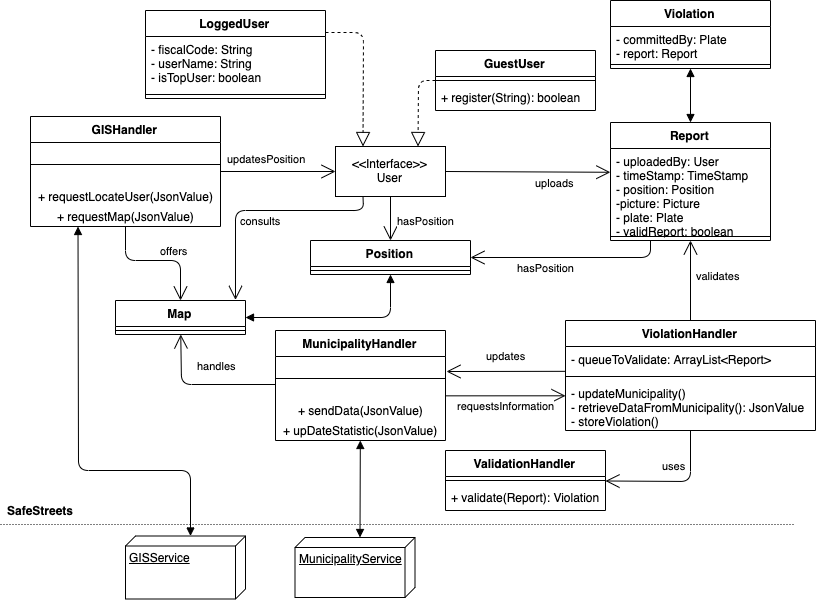
\includegraphics[width=350pt, height=200pt]{diagrams/uml.png}
			\caption{ 
				\label{fig:classDiagram} 
				SafeStreets Class Diagram
			}
		\end{figure}
		
	\subsubsection{System Interfaces}
	\label{sec:systemInterfaces}
		The system requires some external interfaces (represented in \autoref{fig:systemInterfaces}) to accomplish the \hyperref[sec:goals]{goals stated before}. \newline 
		\begin{figure}[h]
			\centering
			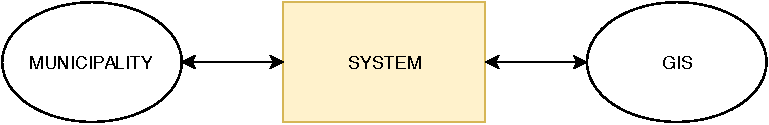
\includegraphics[width=300pt, height=50pt]{diagrams/system_blocks}
			\caption{
				\label{fig:systemInterfaces} 
				Overview of system interfaces
			}
		\end{figure} 
\clearpage			
\paragraph{Municipality Data Exchange} The system will interact with municipalities. The system will retrieve the information about the accidents that occur on the territory of the municipality and cross this information with its own data to identify potentially unsafe areas. It will also retrieve the information about issued tickets from the municipalities to build statistics, for example about the effectiveness of the SafeStreets initiative (e.g., by looking for trends in the issuing of tickets). In addition, our system will expose via a \emph{restricted access API} the stored information about the violations to the municipalities, so that the local authorities can generate traffic tickets from it, and receive suggestions for possible interventions (e.g., add a barrier between the bike lane and the part of the road for motorised vehicles to prevent unsafe parking). \cite{Assignments}


\label{gis}	
\paragraph{Geographic Information System} The system will interact with an external GIS. Our system will map the spatial location of stored violations and visualise the spatial relationships among them. The external GIS will map quantities, such as where the most and least number of violations occurred, to find places that meet the user requested criteria inside an area of interest. This can be accomplished mapping concentrations, or a quantity normalised by area or total number. The system can map the change in a specific geographic area to visualise statistics, or to evaluate the results of the SafeStreets initiative.	

\subsubsection{User Interfaces}
\label{sec:userinterfaces}

The system requires a user interface as the access point where users interact with the system. As the user interface design can dramatically affect the usability and user experience of the system, the layout of the user interface will be clearly set out so that elements can be found in a logical position, in a way that users will be able to find the the information and services they are looking for.

\paragraph{Guest User}
	Using the user interfaces of the system guest users can:
	\begin{itemize}
		\item Register to the system
		\item Authenticate and log-in to the system
	\end{itemize}
	
\paragraph{Logged User}
	Using the user interfaces of the system logged users can:
	\begin{itemize}
		\item Submit a violation with all the required and optional metadata
		\item Consult a map through an external GIS visualising specific data based on a selected criteria
		\item Consult different statistics generated upon the system and the municipality collected data
		\item View and edit personal information
	\end{itemize}
		
\subsubsection{Hardware Interfaces}
\label{sec:hardwareinterfaces}
	The system will interact with the user's device hardware interfaces.	
	\begin{itemize} 
		\item Telephony and other wireless connections are leveraged for the communication between the user and the system
		\item Full access to the user's device camera hardware is needed for the user to capture a photo
		\item The geomagnetic field sensor and the proximity hardware-based sensor are leveraged to determine the position of the user's device
	\end{itemize}

\subsubsection{Software Interfaces}
	In order to accomplish the \hyperref[sec:goals]{goals stated before} the system requires to interface with Databases and DBMSs, required in order to store data about users, violations, and the corresponding metadata. These interfaces are also required to guarantee the ability to input queries to the database in order to satisfy the system required capabilities.
	
\subsubsection{Communication Interfaces}
	The system requires secure communication within the involved entities in a way not susceptible to eavesdropping or interception. Secure communication includes means by which the system can share information that third parties cannot intercept or alter. For these reasons communication encryption methods must be implemented in a way that guarantees the use of encryption, i.e. if encrypted communication is impossible then no traffic is sent.

\subsection{Product Functions}
\paragraph{Violation Upload Procedure} 
Provide logged users with the ability to notify authorities when traffic violations occur and, in particular, parking violations. The application allows users to send pictures of violations, including the suitable required metadata. In particular, when it receives a picture, it runs an algorithm to read the license plate number (the user can help with the recognition via an optional form) and it stores the retrieved information with the violation, including also the type of the violation (submitted by the user) and the street where the violation occurred. \cite{Assignments}

\clearpage

	\begin{figure}[h]
		\centering
		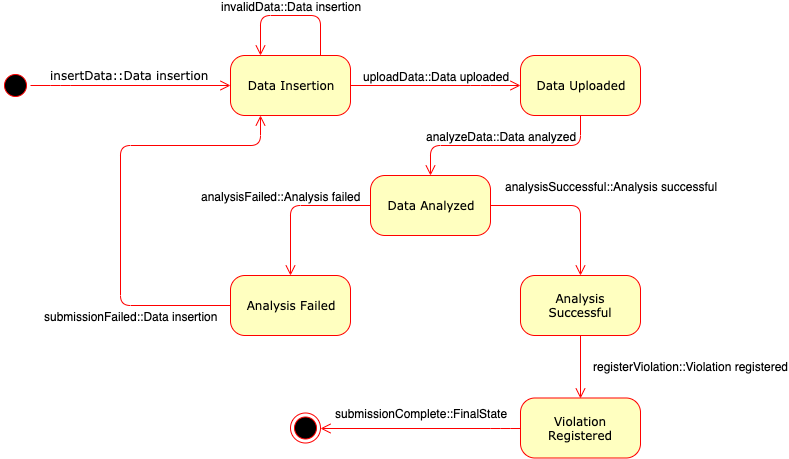
\includegraphics[width=320pt]{diagrams/state-diagrams/SubmitViolation.png}
		\caption{
			\label{fig:violationUpload} Violation Upload Process
		}
	\end{figure}
	
\paragraph{Retrieve Data from Municipality}
Retrieve the information about the accidents that occur on the territory and the issued tickets using the service offered by the municipalities and cross this data with SafeStreets data to identify potentially unsafe areas and build different types of statistics. This will also allow the system to understand which violations are more likely to cause accidents in a particular zone and elaborate suggestions on possible interventions, later communicated to the municipality via a \emph{restricted access API} provided to them. \cite{Assignments} \newline

	\begin{figure}[h]
		\centering
		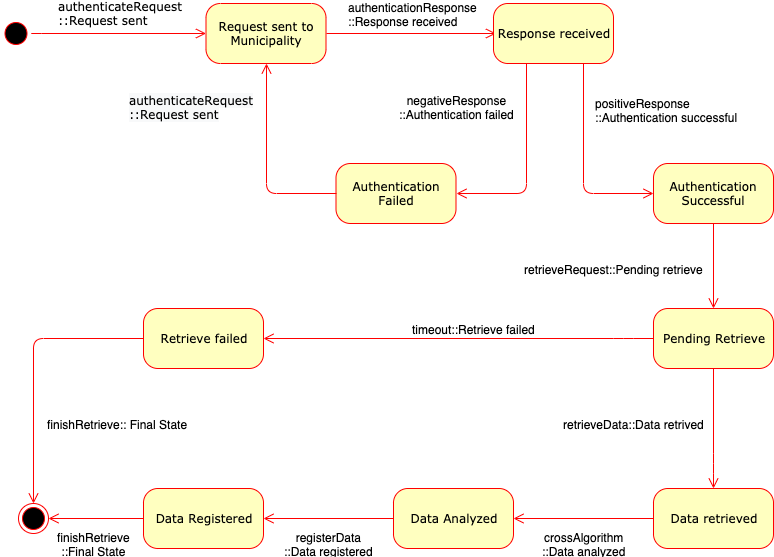
\includegraphics[width=285pt, height=205pt]{diagrams/state-diagrams/RequestMunicipality.png}
		\caption{
			\label{fig:retrieveMunicipality} Retrieve Data From Municipality}
	\end{figure}
	
\clearpage

\paragraph{Show Information and Statistics}
The application allows logged users to mine the information that has been received, highlighting the streets (or the areas) with the highest frequency of violations, considered unsafe areas, or the vehicles that commit the most violations. In addition, statistics about issued tickets, or the effectiveness of the SafeStreets initiative, are shown to the user if requested. \cite{Assignments} \newline
	\begin{figure}[h]
		\centering
		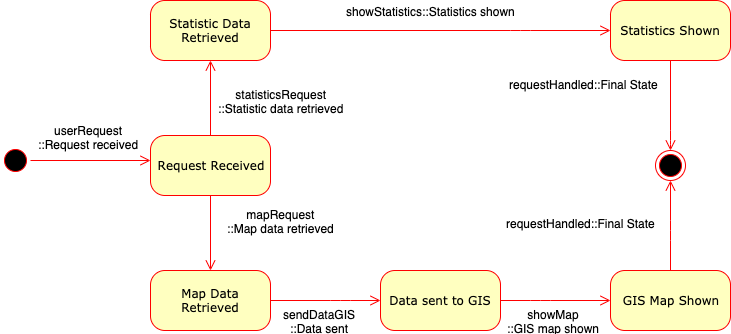
\includegraphics[width=300pt, height=135pt]{diagrams/state-diagrams/ShowStatistics.png}
		\caption{
			\label{fig:showStatistics} Show Information and Statistics
			}
	\end{figure}
	
\paragraph{Restricted Access API}
The system will expose via a \emph{restricted access API} the stored information about the violations to the municipalities, so that the local authorities can generate traffic tickets from it and receive suggestions for possible interventions to carry out (e.g., add a barrier between the bike lane and the part of the road for motorised vehicles to prevent unsafe parking), in order to decrease the risk of those areas, increasing their safety. \cite{Assignments} \newline
	\begin{figure}[h]
		\centering
		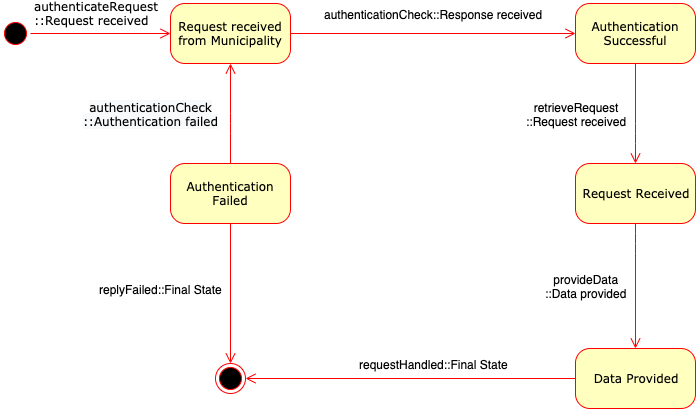
\includegraphics[width=300pt, height=170pt]{diagrams/state-diagrams/RequestAPI.png}
		\caption{
			\label{fig:restrictedAPI} Restricted access API
		}
	\end{figure}


\subsection{User Characteristics}
	Users can use our system when they notice a violation and want to communicate it to the authorities. Necessary conditions for the user in order to use the system are:
 	\begin{itemize}
 		\item The user must have a smartphone with a working connection to the internet and must be able to functionally use the provided services
 		\item The user must be in the age of majority in order to decrease the cases of wrong reports caused by user's inexperience on the topic 
 		\item A direct consequence of the previous item is that the user must be able to identify violations and the different types of violations
 	\end{itemize}
 	The user agrees to these conditions during the registration to the system.
 	
\subsection{Constraints}
\label{sec:constraints}
	We assume that these constraints are always met:
	\begin{enumerate}[label=\textbf{C\arabic*}]
		\item \label{constraint:accurateGPS} GPS position is supposed to be accurate (max error $\pm5$m)
		\item \label{constraint:pictureQuality} The quality of the picture is sufficient to recognise the plate number (min resolution 320x240)
		\item \label{constraint:strongConnection} Internet connection must be strong enough to allow the upload of the picture in a reasonable amount of time (supported technologies are 3G, 4G and 5G due to the performance requirement)
	\end{enumerate}
	
\subsection{Assumptions}
	We assume that these assumptions hold true in the domain of our system 
	\begin{enumerate}[label=\textbf{	DA\arabic*}]
		\item \label{assumption:obtainableGPS} GPS position of all users is always obtainable
		\item \label{assumption:workingConnection} Internet connection always works correctly
		\item \label{assumption:municipalityReachable} Municipality services are always reachable
		\item \label{assumption:mapsReachable} The maps provided by the GIS are always reachable and up to date
		\item \label{assumption:workingDBMS} The DBMS always works properly and the information in the DB are always accessible
		\item \label{assumption:smartphoneOS} The smartphone of the user runs iOS (9 or later) or Android (Jelly Bean or later)
		\end{enumerate}
		
\clearpage

\section{Specific Requirements}

\subsection{External Interfaces}

\subsubsection{System Interfaces}

\paragraph{Municipality Data Exchange} The definition of the municipality data exchange interface is dependent to the corresponding SafeStreet's interface required to be offered to the municipalities. The municipality is required to offer the following functionalities to the system:

	\begin{itemize}
		\item guarantee a secure authentication to the municipalities' system using a provided \emph{restricted access API}
		\item provide a secure transfer of data related to accidents occurred in the territory of the municipality
		\item provide a secure transfer of data related to local authorities' issued tickets 
	\end{itemize} 
	
	Leveraging the retrieved municipality data the system is required to cross this information with the system previously stored data. In addition, the system is required to perform the following functions on the crossed data:
	
	\begin{itemize}
		\item build statistics on the frequency of violations
		\item build statistics on the vehicles that commit the most violations
		\item build statistics on the most egregious offenders leveraging the issued tickets data
		\item build statistics on the effectiveness of the SafeStreets initiative by looking for trends in the issuing of tickets
		\item identify potentially unsafe areas and store this new generated information 
		\item identify possible interventions to be suggested to the municipalities and store this new generated information 
	\end{itemize}
		
	To fulfil the bidirectional data exchange the system is required to offer the following functionalities to the municipalities:
	
	\begin{itemize}
		\item guarantee a secure authentication to the system using a provided \emph{restricted access API}
		\item provide a secure transfer of data related to user uploaded violations and all the corresponding metadata
		\item provide a secure transfer of data related to possible interventions suggestions 
		
	\end{itemize} 
	
\clearpage

\paragraph{Geographic Information System} The definition of the external GIS interface is GIS dependant and will be described in a functionality-based way. The system is required to perform the following functions:

	\begin{itemize}
		\item load and filter data based on the user requested criteria
		\item cache retrieved data for the most common user requested criteria
		\item communicate the loaded and filtered data to the external GIS with the final goal of presenting the requested map to the user via the user interfaces
		
		\end{itemize}
	
	The system via the external GIS is required to be capable of handling the following data visualisations:
	
	\begin{itemize}
		\item visualise the spatial location of stored violations inside a specific geographic area requested by the user
		\item visualise the spatial location of stored violations inside a specific geographic area and a specific time range requested by the user
		\item visualise the distinction between possible safe and unsafe areas identified by the system
		\item map quantities and concentrations, such as where the most and least number of violations occurred, highlighting the streets (and areas) with the highest frequency of violations
		\item map the change of quantities and concentrations inside a specific geographic area and a specific time range requested by the user
	\end{itemize}

	\begin{figure}[h]
		\centering
		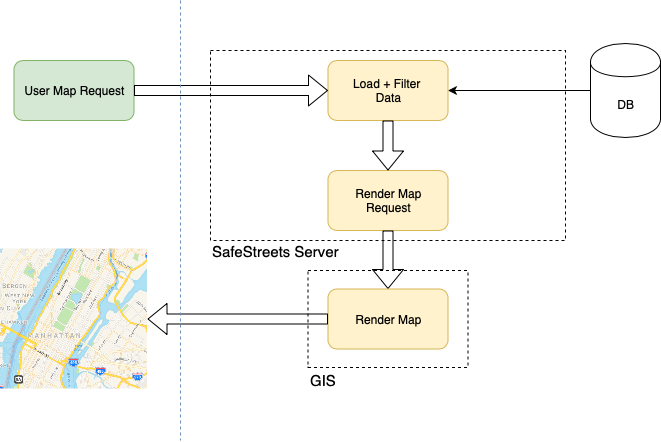
\includegraphics[width=320pt]{diagrams/GIS.png}
		\caption{
			\label{fig:externalGIS} GIS Interaction Diagram}
	\end{figure}

\subsubsection{User Interfaces}
\label{sec:userinterface}

\subsubsection{Hardware Interfaces}
\subsubsection{Software Interfaces}
\subsubsection{Communication Interfaces}


\subsection{Functional Requirements}
Definition of use case diagrams, use cases and associated sequence/activity diagrams, and mapping on requirements

\subsection{Performance Requirements}

\subsection{Logical Database Requirements}

\subsection{Design Constraints}

\subsubsection{Standards Compliance}
\subsubsection{Hardware Limitations}
\subsubsection{Other?}

\subsection{Software System Attributes}

\subsubsection{Reliability}
\subsubsection{Availability}
\subsubsection{Security}
\subsubsection{Maintainability}
\subsubsection{Portability}





\subsection{Functional Requirements}
The following requirements are derived in order to achieve the specified goals.
\subsubsection{Goals}
	\begin{description}
		\item \ref{goal:register}\ Allow guest users to register to the system
			\begin{enumerate}[label=\textbf{R\arabic*}]
			
  				\item The system must require the \emph{guest} user to insert his fiscal code, a username, a valid e-mail and a password to identify him
  				
   				\item The system must check that the validity of the data inserted by the \emph{guest} user namely avoid duplicates, invalid fiscal codes and too weak passwords
   				
   				\item The system must send an e-mail to the \emph{guest} user to verify the e-mail address given during the registration
   
  			\end{enumerate}
  				
				\textbf{DA2} Internet connection always works correctly
				
				\textbf{DA6} The smartphone of the user runs iOS (9 or later) or Android (Jelly Bean or later)
			
  			
		\item \ref{goal:login}\ Allow registered users to authenticate to the system
			\begin{enumerate}[label=\textbf{R\arabic*}, resume]
  				\item The system must require the user to insert his username and password to authenticate to the system
   				\item The system must be able to check if the username and password pair correspond to a user correctly registered to the system and grant the access to that user

			\end{enumerate}
			
			\textbf{DA2} Internet connection always works correctly
			
			\textbf{DA5} The DBMS always works properly so that the information in the DB are always accessible
			
		\item \ref{goal:userTransfer}\ Allow users to transfer data to the system describing occurred violations, including the suitable metadata to describe the submitted violation			\begin{enumerate}[resume*]
				\item The system must allow the user to take a picture of the violation and the plate from the mobile application
  				\item The system must allow the user to manually insert the license plate number in order to help the recognition algorithm
  				\item The system must be able to retrieve the license plate of the vehicle running an algorithm to recognise it
  				\item The system must be able to verify that the license plate number is valid and registered to a vehicle
  				\item The system must require the user to specify the type of violation
  				\item The system must allow the user to provide the location of the violation, manually specifying the address, picking it up from the map or using the GPS of the device
   			\end{enumerate}
   			
   			\textbf{C2} The quality of the picture is sufficient to recognise the plate number (min resolution 320x240)
   			
			\textbf{C3} Internet connection must be strong enough to allow the upload of the picture in a reasonable amount of time (supported technologies are 3G, 4G and 5G due to the performance requirement)
			
			\textbf{DA1} GPS position of all users is always obtainable
			
			\textbf{DA2} Internet connection always works correctly
			
		\item \ref{goal:avoidLeaks}\ Ensure that the chain of custody of the information provided by the users is never broken, and the information is never altered or manipulated			\begin{enumerate}[resume*]
   				\item The system must provide a secure channel to communicate with the users
   				\item The system must encrypt the connection with the users in order to protect the process of providing data
   				\item The system must adopt security measures to prevent malicious accesses and to protect sensible data
   				\item Questo davvero non lo so mori miei
  			\end{enumerate}
  			
  			
		
		\item \ref{goal:municipalityTransfer}\ Allow the system to retrieve data about the accidents that occur on the territory and data about issued tickets via the municipality provided service
			\begin{enumerate}[resume*]
   				\item The system must be able to retrieve data about accidents from municipality systems 
   				\item The system must be able to process data retrieved from municipality
   				\item The system must be able to elaborate accidents and violations information to extract data about unsafe areas
   				\item The system must be able to provide data to municipality systems to suggest possible interventions to increase safety in a specific area
  			\end{enumerate}
  			
  			\textbf{DA2} Internet connection always works correctly
  			
			\textbf{DA3} Municipality services are always reachable
  			
  		\item \ref{goal:statistics}\ Allow the system to cross the information submitted by the users and the information retrieved from the municipality to build statistics
  			\begin{enumerate}[resume*]
  				\item 
   				
  			\end{enumerate}
  		\item \ref{goal:consultMap}\ Allow users to consult a map highlighting the streets (and the areas) with the highest frequency of violations, the identified potentially unsafe areas and view statistics about previously stored violations
  			\begin{enumerate}[resume*] 
  				\item The system must be able to retrieve data about tickets issued by the municipality 
   				\item The system must be able to process data retrieved from municipality
   				\item The system must be able to elaborate issued tickets information to generate statistics about useful violations provided by users
   			\end{enumerate}
   			
   			\item \ref{goal:retrieveData}Allow municipality to consult the system data and receive suggestions on possible interventions via a restrict access API 
   				\begin{enumerate}[resume*] 
  				\item The system must be able to retrieve data about tickets issued by the municipality 
   				\item The system must be able to process data retrieved from municipality
   				\item The system must be able to elaborate issued tickets information to generate statistics about useful violations provided by users
   			\end{enumerate}
   			
   	\end{description}
  	
\subsection{Performance Requirements}
	The system should ensure acceptable response times in the interactions with the user, which strictly depends on the number of concurrent users and the connection speed.
\newline
The processes of providing data and loading the map of safe and unsafe areas shouldn't be too slow.
\subsection{Software System Attributes}
	\subsubsection{Availability}
	The system must be available 99,9\% of the time (up to 8,76 hours per year of downtime). The system should be accessible 24 hours per day.
	\subsubsection{Security}
	Users personal information and payment information are encrypted and must be protected during transmission, as already stated the PTPP protocol will be used to ensure encryption through the network.
	Restricted access APIs must check that who tries to use them is actually allowed to do so.
	\subsubsection{Portability}
	The system must be also accessible by the most common mobile platforms (iOS and Android devices).



\section{Use cases identification}
\subsection{Scenarios}
Here are some scenarios that describe the usage of the system.
\subsubsection{Scenario 1}
\label{scenario:1}
	Davide is walking down the street and notices a car parked over the crosswalks. He opens the SafeStreets app, registers to the system with his fiscal code, and takes a picture from the in-app camera. Before uploading he adds information such as the type of violation (i.e. "Bad Parking") and the street in which the violation occurred. As soon as SafeStreet processes the uploaded data the authorities are alerted.

\subsubsection{Scenario 2}
\label{scenario:2}
	Carlo wants to teach his son to drive and wants to find the safest area of Isernia in order to avoid exposing him to difficult situations in his first drives. He opens the SafeStreets app and consult the map with the streets that have the greatest number of incidents and violations, and will try to avoid them allowing his son to have a safe drive.

\subsubsection{Scenario 3}
\label{scenario:3}
	SafeStreets automatically retrieves data from the municipality's service, and after a while notices that extremely frequently cars are parked in a restricted area of Milan. After further analysis and with the help of the users they come to the conclusion that don't realise that they can't park in that area because of a misleading signal, so they contact the municipality and offer a possible solution to the problem.

\subsubsection{Scenario 4}
\label{scenario:4}
	After receiving a notification of "Dangerously parked car" with the picture showing a car parked in such a way that could risk a possible collision with the tram line, SafeStreets alerts the authorities in order to facilitate the process of car removal and the consequential ticket generation.

\subsubsection{Scenario 5}
\label{scenario:5}
	\todo{picture rejection?}
	
\subsubsection{Scenario 6}
\label{scenario:6}
	Non so more ce ne verranno altri

\clearpage
\subsection{Use case diagram}

\begin{figure}[h!]
	\centering
	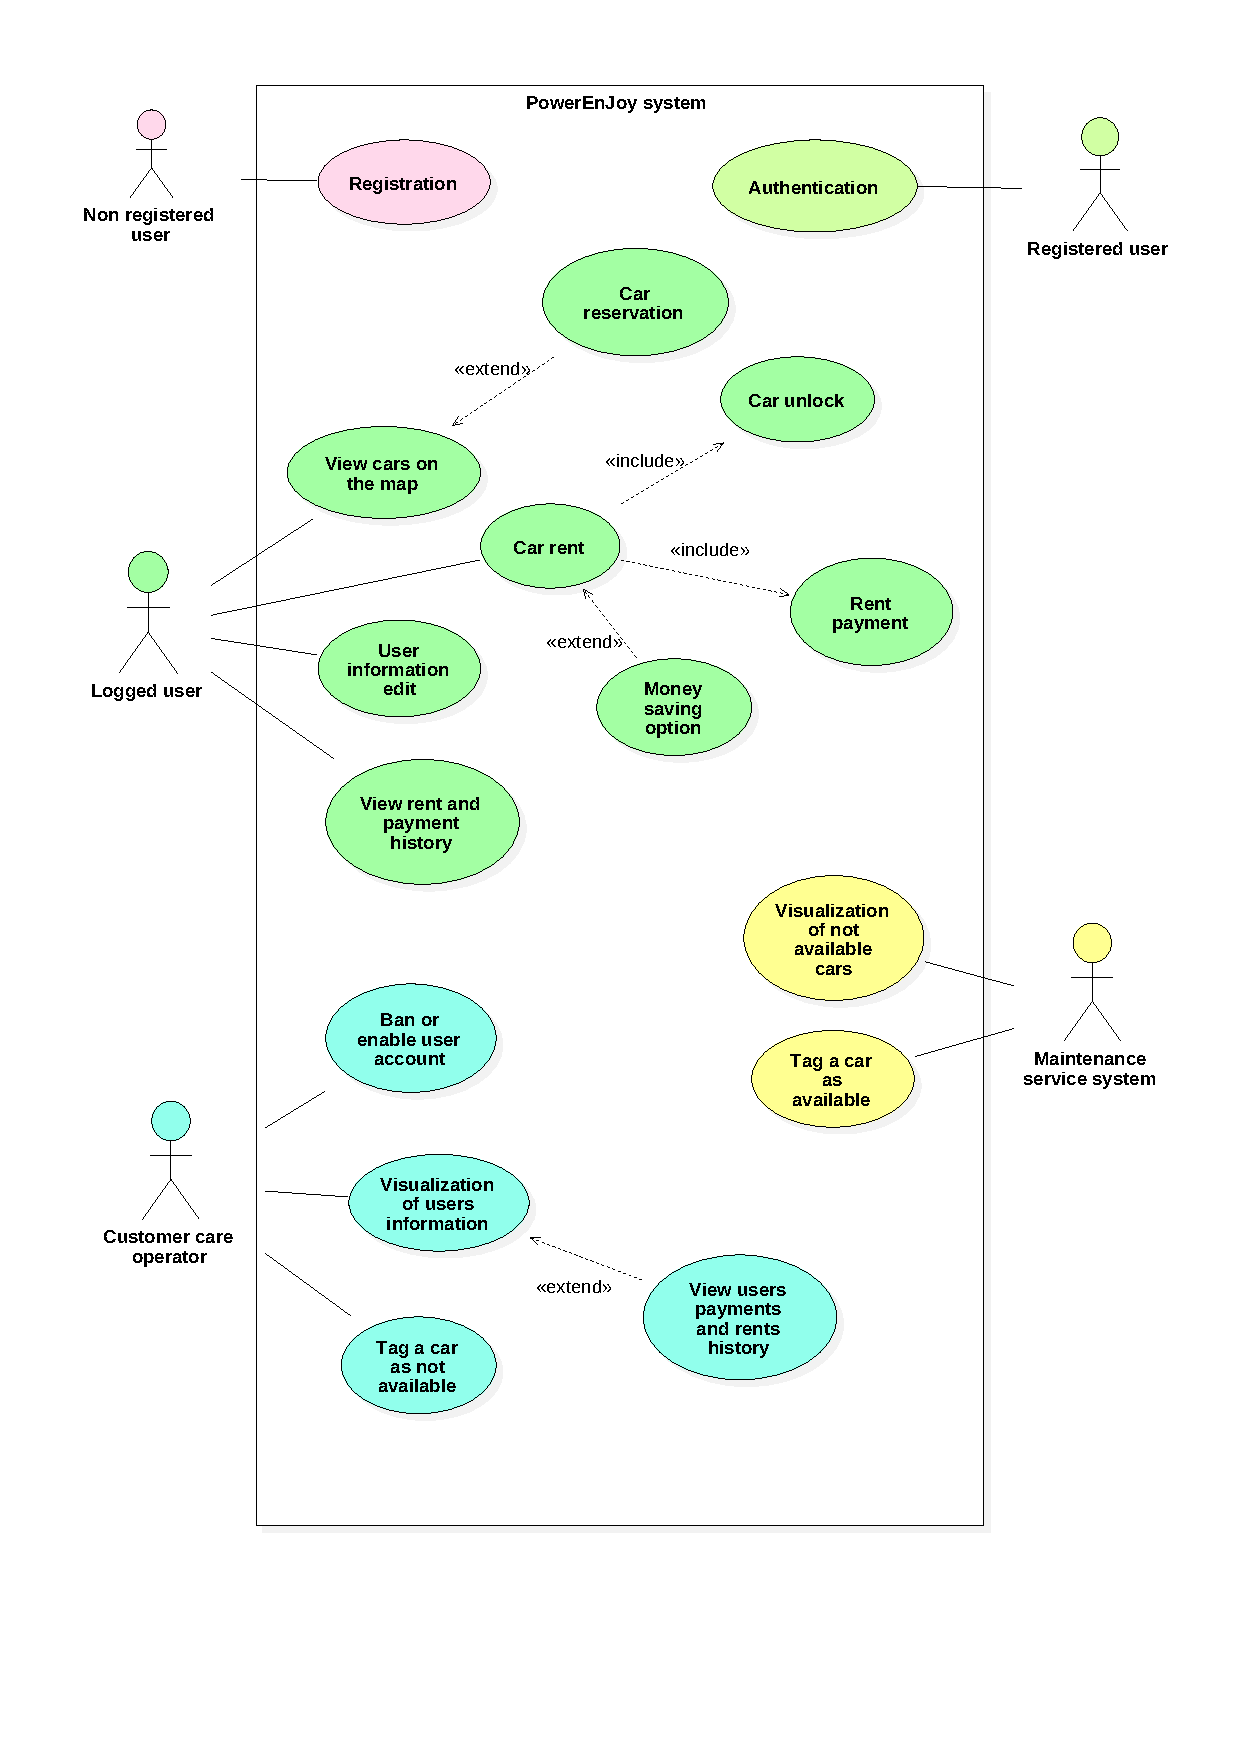
\includegraphics[width=\linewidth]{useCase}
	\caption{
		\label{fig:useCase} 
		Use case diagram
	}
\end{figure}
\clearpage
\paragraph{Notes to read the diagram}
The use case diagram represents the possible interactions of actors with the system and the different use cases in which the actors are involved.\\

The "Maintenance service system" is an external software which the system-to-be needs to interact with. \\
 
We do not consider the external payment handling system an actor since it does not start any interaction with our system, it simply reacts when our system requests its services; this interaction is encapsulated as sub-procedure in the flow of events of the "Rent payment" use case.\\

We do not consider the car an actor for the same reason, moreover the only interactions started by the car are trigger events which are very simple interactions, which we do not consider use cases.\\
\clearpage
\subsection{Use cases description}

\subsubsection{Registration}
\begin{longtable}{p{0.25\linewidth}p{0.75\linewidth}}
\toprule
\textbf{Name} & \textbf{Registration} \\
\midrule
\textbf{Actors} & Non registered user \\
\midrule
\textbf{Entry conditions} & \\
\midrule
\textbf{Flow of events} & 
\begin{enumerate}
	\item The user asks the system to register to its services
	\item The system shows the appropriate form to fill to register to the system
	\item The user inserts an username to be uniquely identified by the system
	\item The user inserts his own email address
	\item The user inserts his name, surname, birth date and place and current domicile
	\item The user inserts his driving license ID code
	\item The user inserts payment information
	\item The user confirms data inserted are correct e submit the form
	\item The system checks the username to be unique
	\item The system checks the email to be unique
	\item The system checks the driving license ID to be unique
	\item The system sends an email to the user with a unique link to verify the email address inserted by the user really belongs to him
	\item The user clicking on the link received confirms his email address
	\item The user is notified by mail the registration procedure is correctly completed and
	provided with a password bound to his username to access the system
\end{enumerate} \\
\midrule
\textbf{Exit conditions} & The user is able to authenticate to the system as \emph{registered} user with its own credentials\\
\midrule
\textbf{Exceptions} & 
\begin{itemize}
	\item If the username inserted by the user is already used by another user, the system displays an error message asking the user to insert another username
	\item If the mail inserted by the user is already used by another user, the system displays an error message asking the user to insert another mail
	\item If the user notices to have entered wrong informations he could edit them at the end of the process of registration in his personal page
\end{itemize} \\
\bottomrule
\caption{\emph{Registration} use case description}
\end{longtable}

\begin{figure}[h!]
	\centering
	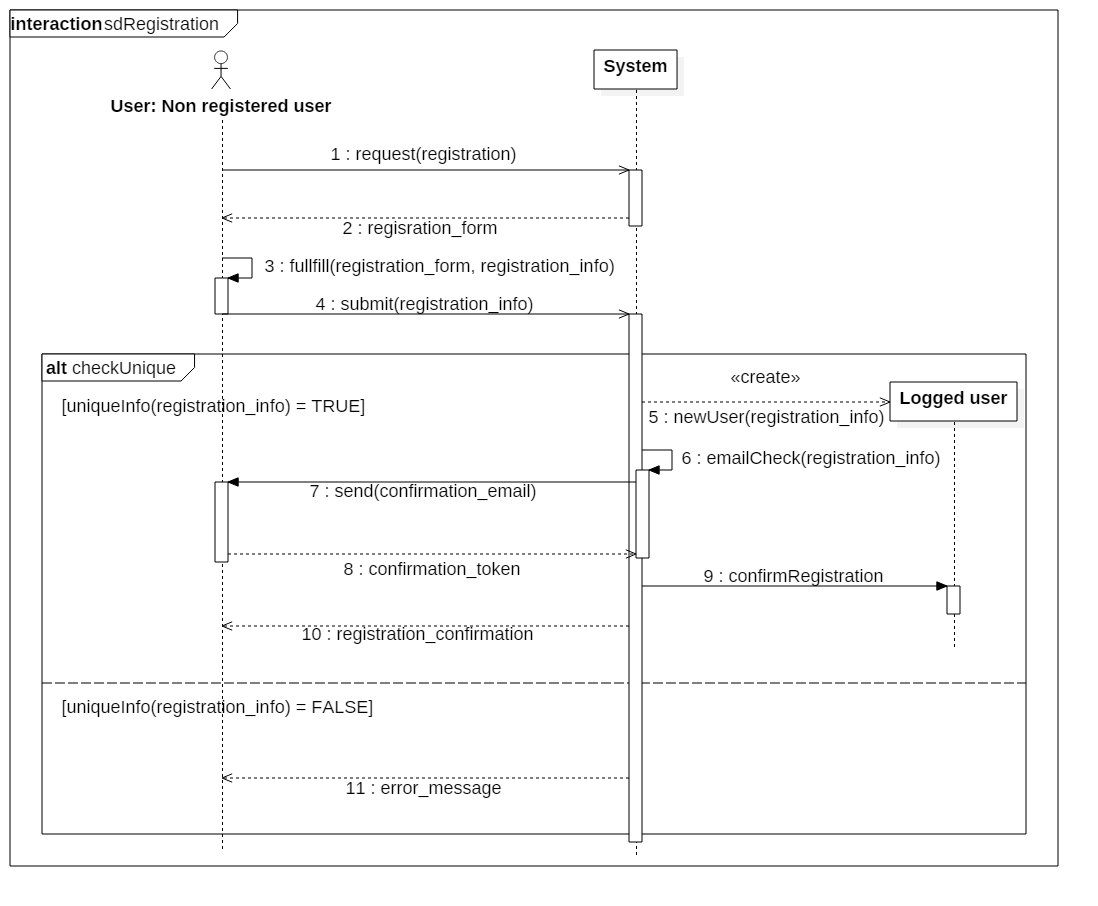
\includegraphics [width=\textwidth]{/diagrams/Sequence/sdRegistration.png}
	\caption{
		\label{fig:registrationSequence} 
		\emph{Registration} sequence diagram
	}
\end{figure}

%///////////////////////////////////////////////////////////
\clearpage
\subsubsection{Authentication}
\begin{longtable}{p{0.25\linewidth}p{0.75\linewidth}}
\toprule
\textbf{Name} & \textbf{Authentication} \\
\midrule
\textbf{Actors} &  Registered user \\
\midrule
\textbf{Entry conditions} & The user must know his username and password \\
\midrule
\textbf{Flow of events} & 
\begin{enumerate}
	\item The user inserts his username and password in the appropriate form and submit it
	\item The system validates the inserted credentials checking also if the user has confirmed his own email address
	\item The system checks if the user is banned
\end{enumerate} \\
\midrule
\textbf{Exit conditions} & If the credential validation is successful and the user is not banned he is granted the proper privileges\\
\midrule
\textbf{Exceptions} & 
\begin{itemize}
	\item If the credential validation failed an error message is displayed
	\item If the credential validation is successful and the user is banned a message providing assistance is displayed and the system doesn't allows the user to access to the system
\end{itemize} \\
\bottomrule
\caption{\emph{Authentication} use case description}
\end{longtable}


\begin{figure}[h!]
	\centering
	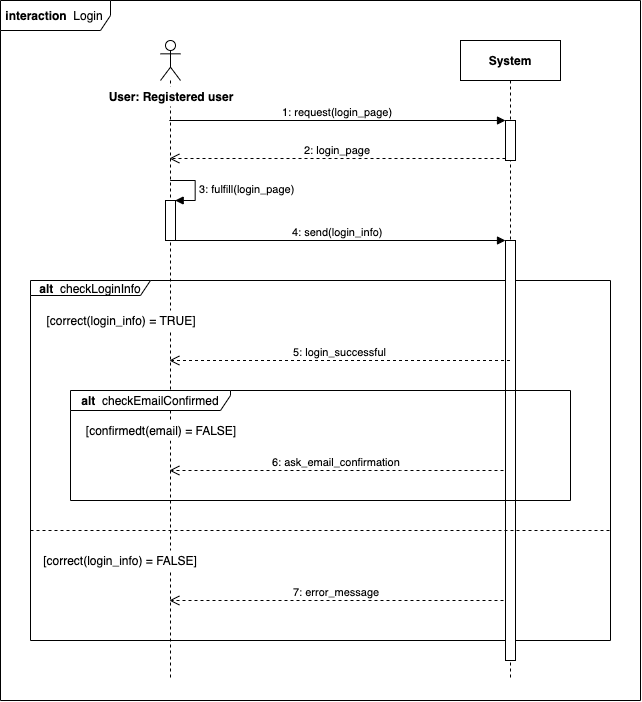
\includegraphics [width=\textwidth]{/diagrams/Sequence/sdLogin.png}
	\caption{
		\label{fig:authSequence} 
		\emph{Authentication} sequence diagram
	}
\end{figure}

%///////////////////////////////////////////////////////////
\clearpage
\subsubsection{View cars on the map}
\begin{longtable}{p{0.25\linewidth}p{0.75\linewidth}}
\toprule
\textbf{Name} & \textbf{View cars on the map} \\
\midrule
\textbf{Actors} &  Logged user \\
\midrule
\textbf{Entry conditions} & \\
\midrule
\textbf{Flow of events} & 
\begin{enumerate}
	\item The user chooses if he wants to use his GPS position or insert a different one manually
		\subitem a. The system retrieves the user's GPS position
		\subitem b. The user inserts a position
	\item The system retrieves the position of all \emph{Available} cars and their battery level percentage
	\item The system shows a map with all available cars, charging stations position and safe areas near the position indicated
	\item The user can click on a car on the map to see its battery level percentage
\end{enumerate}\\
\midrule
\textbf{Exit conditions} & The user can navigate a map with all available cars near the position indicated by him\\
\midrule
\textbf{Exceptions} & 
If the position inserted by the user is not correct an error message is displayed \\
\bottomrule
\caption{\emph{View cars on the map} use case description}
\end{longtable}

\begin{figure}[h!]
	\centering
	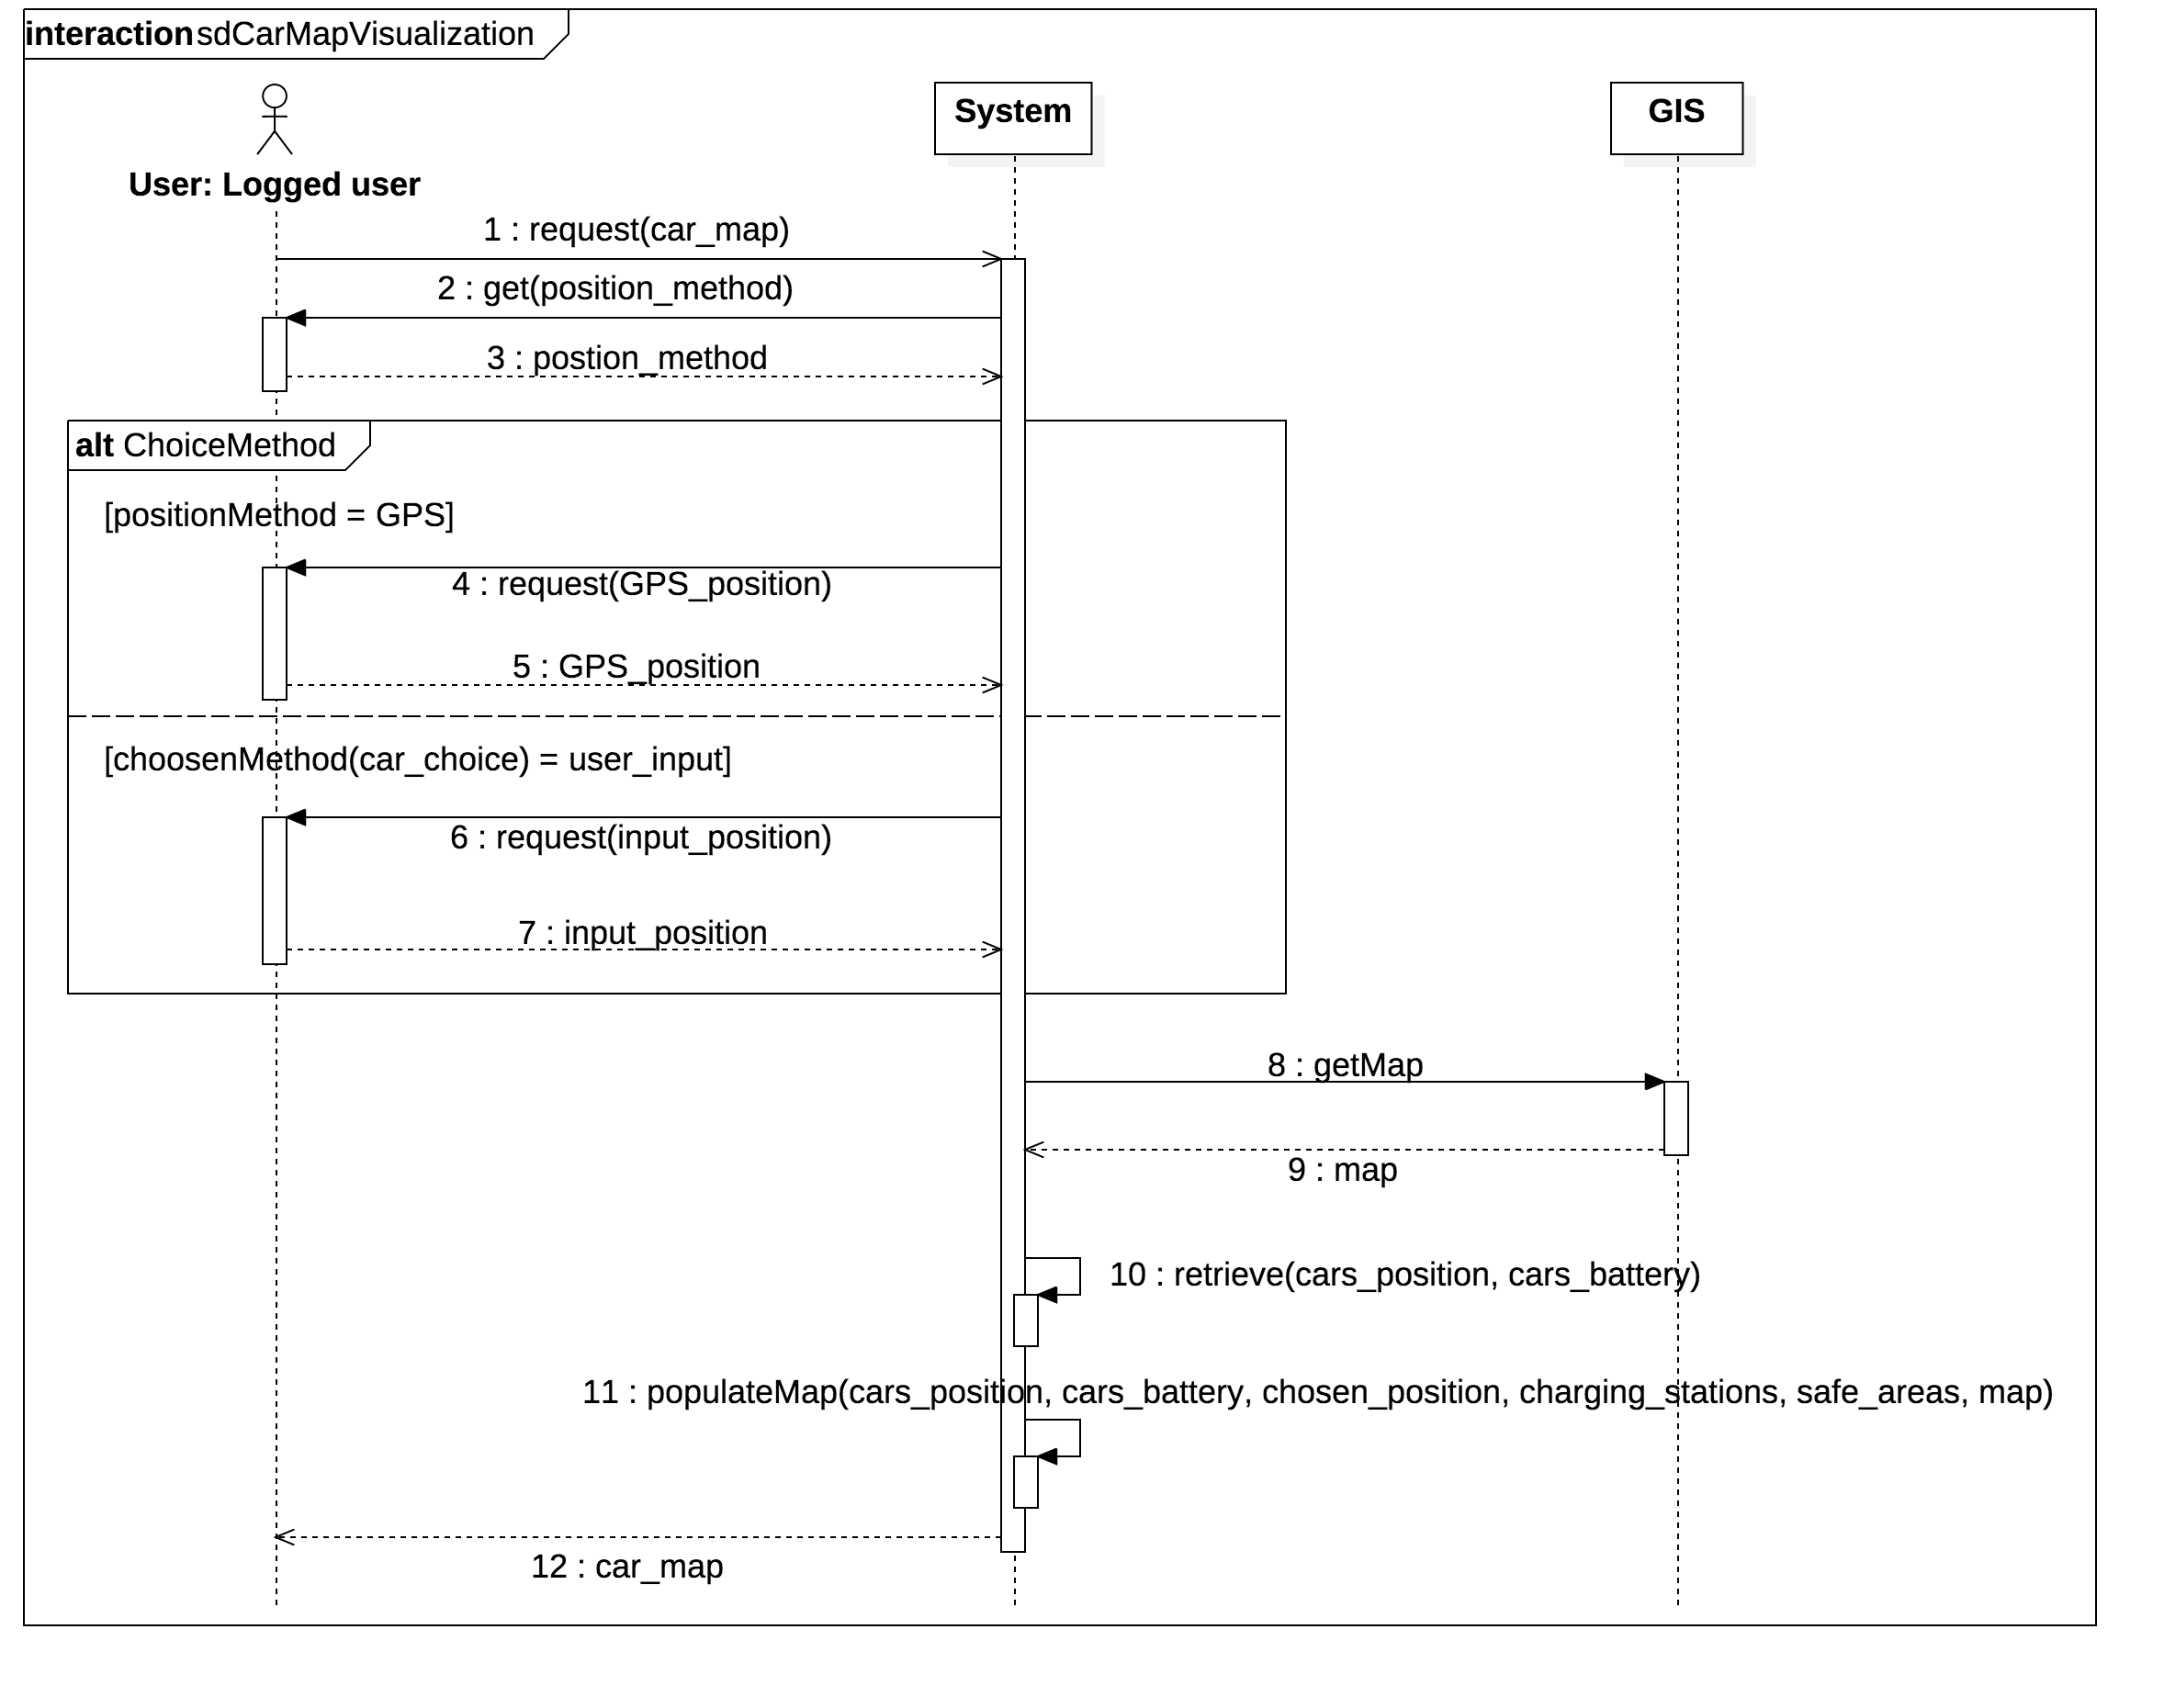
\includegraphics [width=\textwidth]{/diagrams/Sequence/sdCarMapVisualization.png}
	\caption{
		\label{fig:carsMapSequence} 
		\emph{View cars on the map}  sequence diagram
	}
\end{figure}

%///////////////////////////////////////////////////////////
\clearpage
\subsubsection{Car reservation}
\begin{longtable}{p{0.25\linewidth}p{0.75\linewidth}}
\toprule
\textbf{Name} & \textbf{Car reservation} \\
\midrule
\textbf{Actors} &  Logged user \\
\midrule
\textbf{Entry conditions} & \\
\midrule
\textbf{Flow of events} & 
\begin{enumerate}
	\item \textbf{View cars on the map}
	\item The user selects the car he wants to reserve
	\item The user confirms he wants to reserve that car
\end{enumerate}\\
\midrule
\textbf{Exit conditions} & The system set the state of the chosen car as \emph{Reserved} paired with the user who made the reservation\\
\midrule
\textbf{Exceptions} &  If the user has already reserved a car, the system shows an error message and doesn't allow him to reserve another car \\
\bottomrule
\caption{\emph{Car reservation} use case description}
\end{longtable}

%///////////////////////////////////////////////////////////
\clearpage
\subsubsection{Car unlock}
\begin{longtable}{p{0.25\linewidth}p{0.75\linewidth}}
\toprule
\textbf{Name} & \textbf{Car unlock} \\
\midrule
\textbf{Actors} &  Logged user \\
\midrule
\textbf{Entry conditions} & The user reserved car \\
\midrule
\textbf{Flow of events} & 
\begin{enumerate}
	\item The user asks the system to unlock the car he reserved
	\item The system checks if the user's position is at most 5 meters away from the position of the car he reserved
	\item The system unlocks the car with the state set as \emph{Reserved} paired with the aforementioned user
	\item The system sends a message to the user, confirming that the car is unlocked
\end{enumerate} \\
\midrule
\textbf{Exit conditions} & The car is unlocked and the user can pick it up\\
\midrule
\textbf{Exceptions} & 
\begin{itemize}
	\item If the position of the user is not at most 5 meters away from the position of the car he reserved the system displays an error message
\end{itemize} \\
\bottomrule
\caption{\emph{Car unlock} use case description}
\end{longtable}


\begin{figure}[h!]
	\centering
	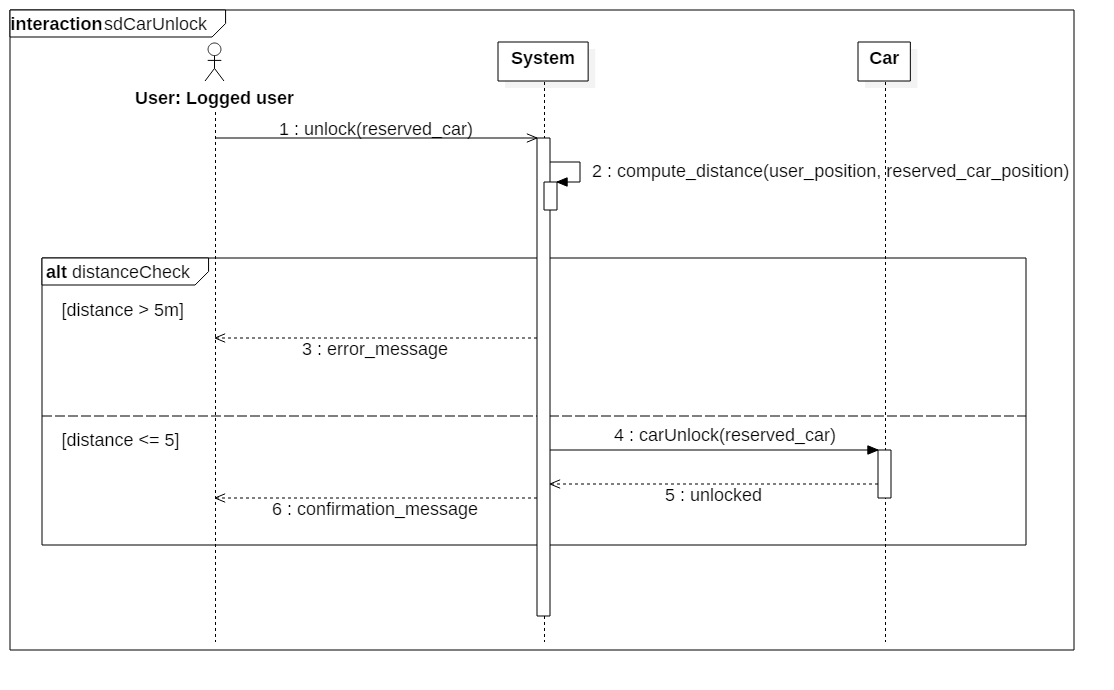
\includegraphics [width=\textwidth]{/diagrams/Sequence/sdCarUnlock.png}
	\caption{
		\label{fig:carUnlockSequence} 
		\emph{Car unlock} sequence diagram
	}
\end{figure}

%///////////////////////////////////////////////////////////
\clearpage
\subsubsection{Car rent}
\begin{longtable}{p{0.25\linewidth}p{0.75\linewidth}}
\toprule
\textbf{Name} & \textbf{Car rent} \\
\midrule
\textbf{Actors} &  Logged user \\
\midrule
\textbf{Entry conditions} & 
The user is paired with the \emph{Reserved} state of a car\\
\midrule
\textbf{Flow of events} & 
\begin{enumerate}
	\item \textbf{Car unlock}
	\item The user ignites the car engine
	\item The system sets the state of the \emph{Reserved} car to \emph{In Use} paired
	with the same user
	\item During the rent the user is informed about the current charge and whether he is or not inside a safe area
	\item The user leaves the car turning off the engine and closing the doors
	\item The system locks the car
    \item The system activates a timer to allow the user to plug the car into a charging station if it is
    near one of them
    \item When the timer expires:
    	\begin{enumerate}[label = 8.\arabic*]
    		\item The system retrieves informations about the ride from the car: number of passengers detected during the ride, position of the car and battery level at the end of the ride and if the car is or not on charge 
    		\item The system sets the car as \emph{Available}
    	\end{enumerate}
    \item \textbf{Rent payment}
\end{enumerate} \\
\midrule
\textbf{Exit conditions} & 
The user is charged of the correct amount for the ride and at anytime could perform another rent, the car is available again\\
\midrule
\textbf{Exceptions} & 
\begin{itemize}
	\item If the user doesn't start the engine up to one hour after the reservation, he is charged of 1\euro (through a payment procedure), the car state is set as \emph{Available} and the user is notified his reservation is expired
\end{itemize} \\
\bottomrule
\caption{\emph{Car rent} use case description}
\end{longtable}

\begin{figure}[h!]
	\centering
	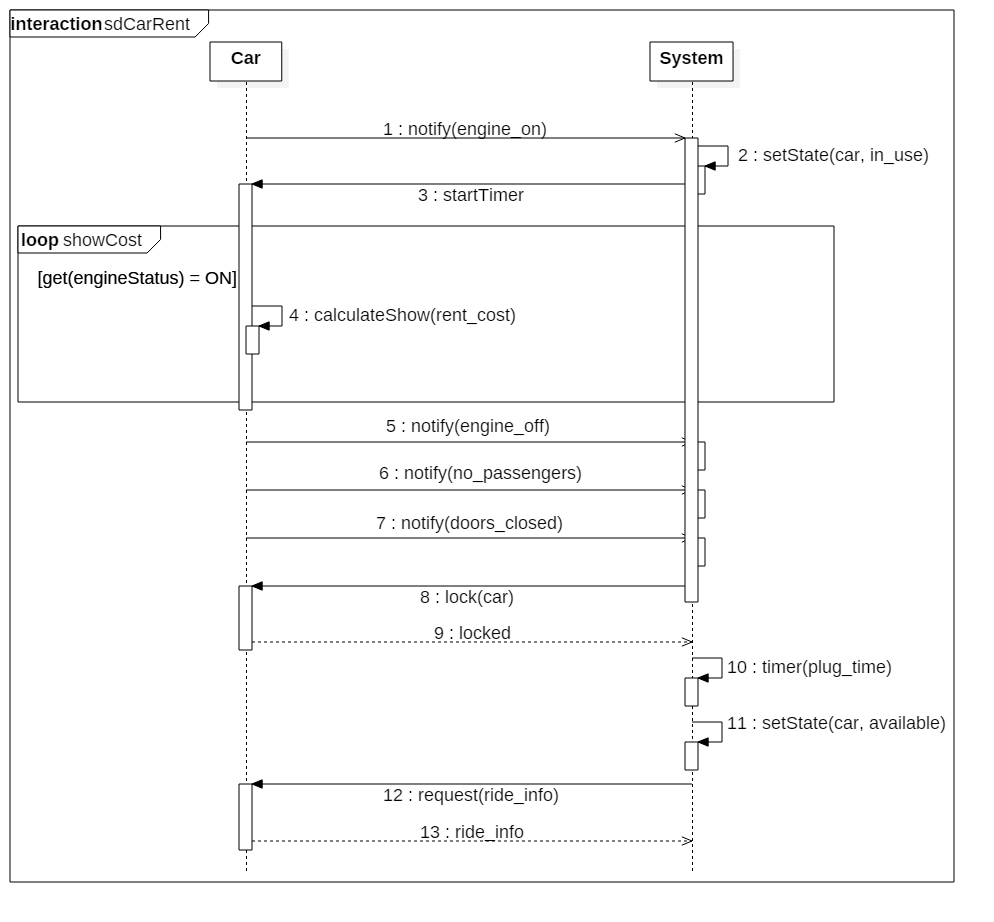
\includegraphics [width=\textwidth]{/diagrams/Sequence/sdCarRent}
	\caption{
		\label{fig:rentSequence} 
		\emph{Car rent} sequence diagram
	}
\end{figure}

\begin{figure}[h!]
	\centering
	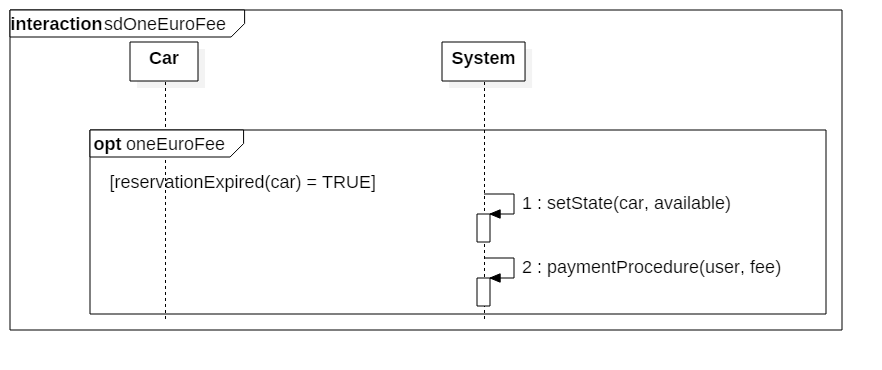
\includegraphics [width=\textwidth]{/diagrams/Sequence/sdOneEuroFee}
	\caption{
		\label{fig:euroFeeSequence} 
		\emph{One Euro fee} sequence diagram
	}
\end{figure}
\clearpage
The overall status of a car can be represented by the FSM in \autoref{fig:carFSA}
	\begin{figure}[h]
			\centering
			\includegraphics[scale=0.5]{CarFSA}
			\caption{
				\label{fig:carFSA} 
				Car status FSM
			}
		\end{figure}
%///////////////////////////////////////////////////////////
\paragraph{Notes to read the diagram}
The \emph{Not Available} state includes the cases in which the car is either broken or a user left it with a critical battery level and not on charge.\\ 

The system changes the state of a car from \emph{Available} to \emph{Not Available} when its battery level is critical and the car is not on charge (see \ref{req:notAvailbleCritical}).\\

Even if the car is left with no battery left, it is still able to communicate with the system, so the rent can end normally and the maintenance service will take care the car
(see \ref{da:zeroBattery}).
\clearpage

\subsubsection{Rent payment}
\begin{longtable}{p{0.25\linewidth}p{0.75\linewidth}}
\toprule
\textbf{Name} & \textbf{Rent payment} \\
\midrule
\textbf{Actors} &  Logged user\\
\midrule
\textbf{Entry conditions} & 
The user must have completed a rent shutting off the engine and exiting the car. The system has retrieved information about the ride from the car. \\
\midrule
\textbf{Flow of events} & 
\begin{enumerate}
	\item The system checks if the car position is or is not inside a safe area
	\item The system checks if the car has detected more than one passenger during the rent
	\item The system checks the car battery percentage
	\item The system checks if the car is plugged on a charging station
	\item The system checks the distance of the car from the nearest charging station
	\item The system calculates the cost of the ride based on the rent time
	\item The system determines the applicable discounts/extra fee applying it to the cost of the ride
	\item The system starts a payment procedure with user's payment information using
	an external service
	\item The system waits a response from the external payment service
	\item The system logs data about the rent and the payment
    \item The system notifies the user about the result of the payment procedure and on discount/extra fees applied
\end{enumerate} \\
\midrule
\textbf{Alternative flow} & 
Flow of events as specified upon from \emph{1} to \emph{7}
\begin{enumerate}[label=8 \alph*.]
	\item The system detects the user has enabled the \emph{money saving option}
	\item The system checks if the car is currently on charge on the charge station determined by the system at the begin of the rent
	\item The system determines the applicable discounts/extra fee applying it to the cost of the ride eventually also taking in account the \emph{money saving option} discount if the car is currently on charge on the charge station determined by the system at the begin of the rent
\end{enumerate}
Flow of events as specified upon from \emph{9} to \emph{12} \\
\midrule
\textbf{Exit conditions} & 
The user is charged of the correct amount for the ride\\
\midrule
\textbf{Exceptions} & 
\begin{itemize}
	\item If the payment procedure is not correctly completed the user is banned, rent information is stored, the payment suspended and the user is informed to contact the customer service.  
\end{itemize} \\
\bottomrule
\caption{\emph{Rent payment} use case description}
\end{longtable}

\begin{figure}[h!]
	\centering
	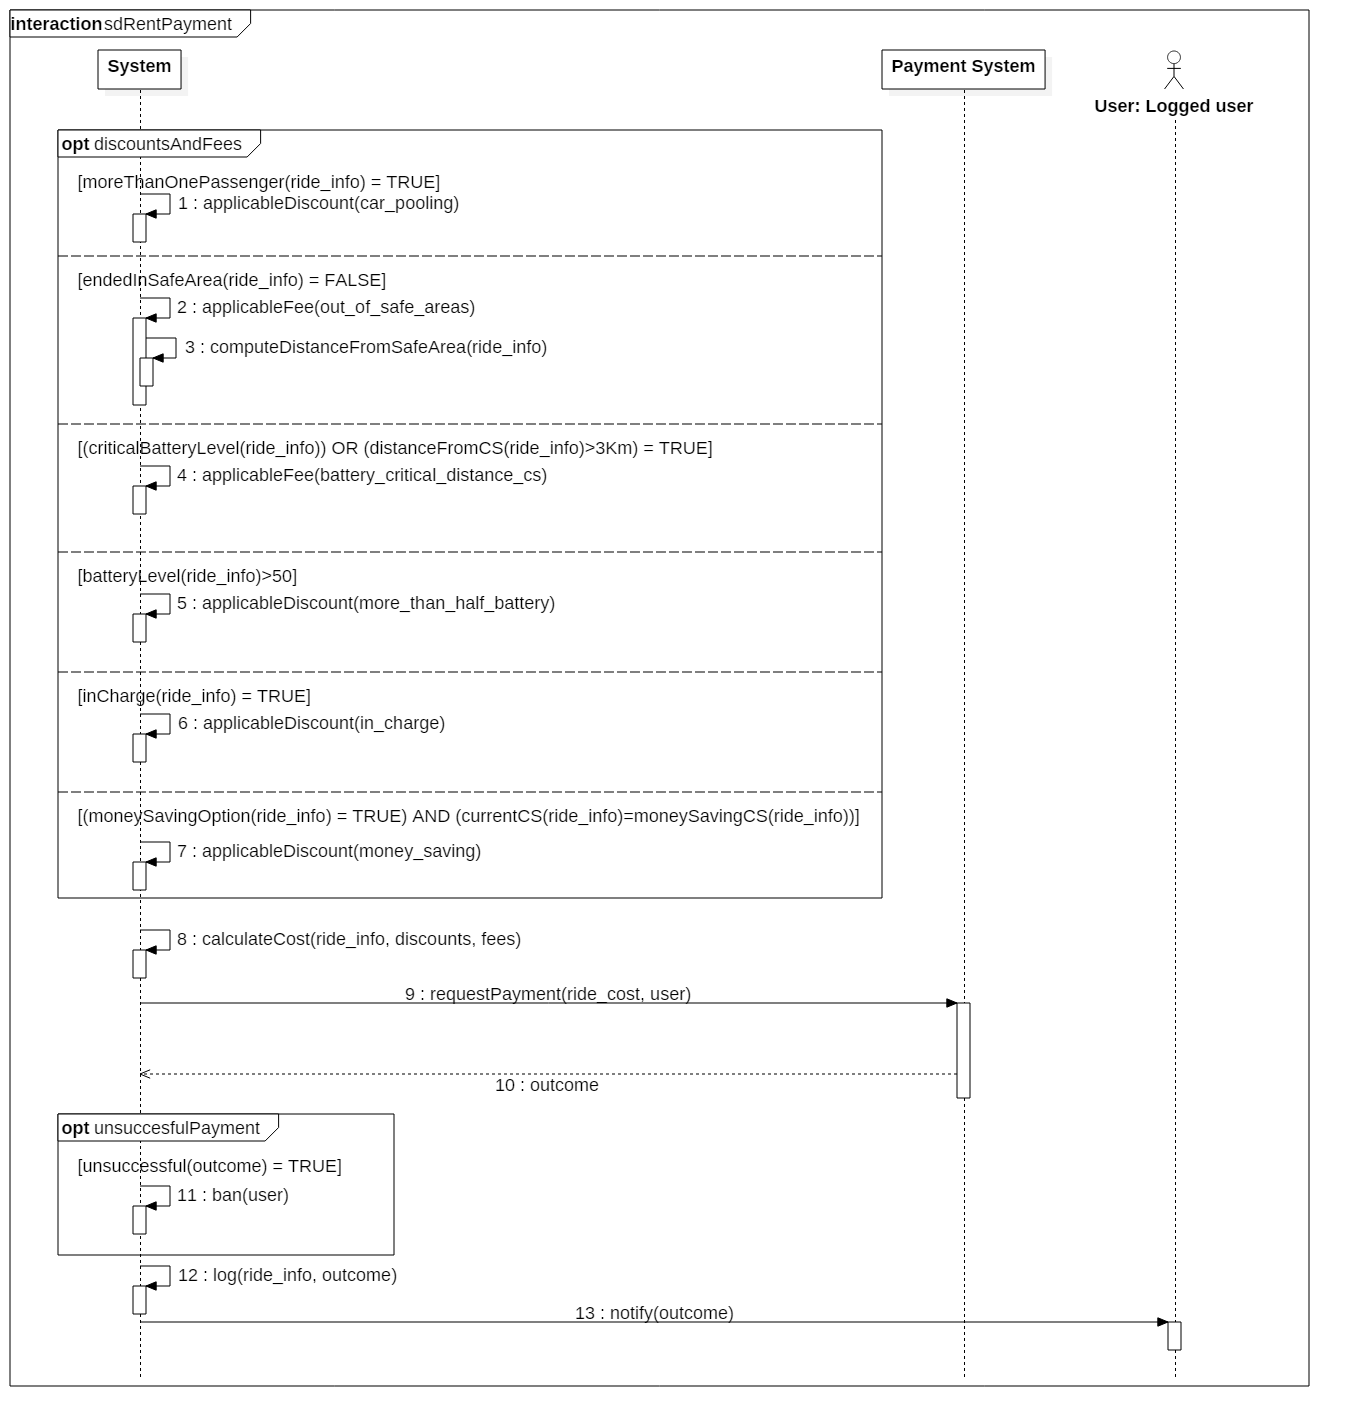
\includegraphics [width=\textwidth]{/diagrams/Sequence/sdRentPayment}
	\caption{
		\label{fig:paymentSequence} 
		\emph{Rent payment} sequence diagram
	}
\end{figure}

%///////////////////////////////////////////////////////////
\clearpage
\subsubsection{Money saving option}
\begin{longtable}{p{0.25\linewidth}p{0.75\linewidth}}
\toprule
\textbf{Name} & \textbf{Money saving option} \\
\midrule
\textbf{Actors} &  Logged user\\
\midrule
\textbf{Entry conditions} & 
The user should have enabled the \emph{money saving option} \\
\midrule
\textbf{Flow of events} & 
\begin{enumerate}
	\item \textbf{Car Reservation}
	\item The system asks the user to insert his destination
	\item The user inserts his destination
	\item The system searches for charging stations near the destination position inserted by the
	user with available plugs
	\item The system chooses a charging station in order to ensure a uniform distribution of cars in
	the city and taking in account the destination of the user
	\item The system informs the user about the charging station to reach in order to obtain the discount
	\item \textbf{Car Rent} (\textbf{Car Reservation} already done)
\end{enumerate} \\
\midrule
\textbf{Exit conditions} &
\begin{itemize}
	\item If the user has left the car plugged in the charging station suggested by the
	\emph{money saving option} he has obtained the correct discount
	\item The user can any time perform another rent
	\item Car is again available
\end{itemize} \\
\midrule
\textbf{Exceptions} & 
\begin{itemize}
	\item If the user doesn't leave the car in the charging station suggested by the
	\emph{money saving option} he doesn't obtain the related discount
\end{itemize} \\
\bottomrule
\caption{\emph{Money saving option} use case description}
\end{longtable}

\begin{figure}[h!]
	\centering
	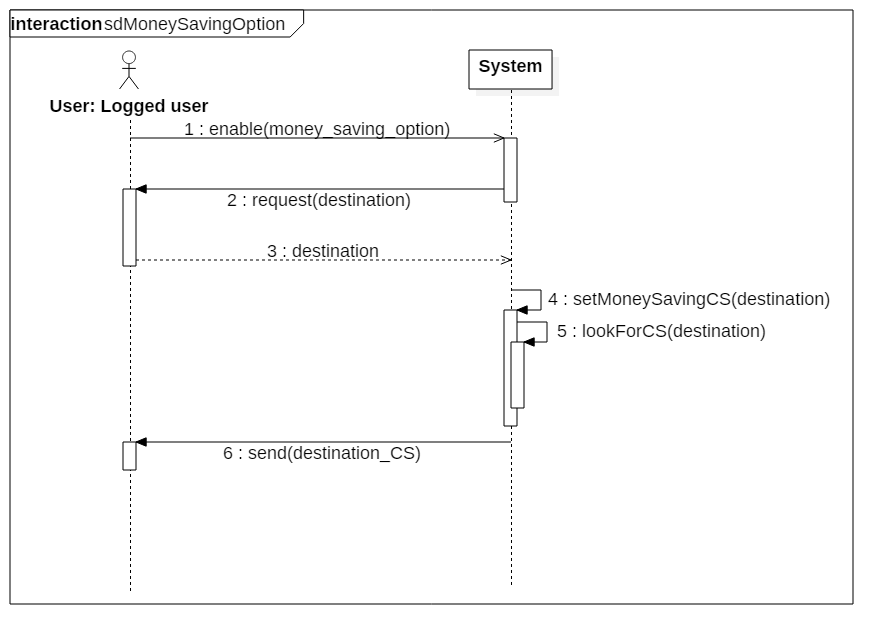
\includegraphics [width=\textwidth]{/diagrams/Sequence/sdMoneySavingOption}
	\caption{
		\label{fig:msOptionSequence} 
		\emph{Money saving option} sequence diagram
	}
\end{figure}

%///////////////////////////////////////////////////////////
\clearpage
\subsubsection{Visualization of not available cars}
\begin{longtable}{p{0.25\linewidth}p{0.75\linewidth}}
\toprule
\textbf{Name} & \textbf{Visualization of not available cars} \\
\midrule
\textbf{Actors} &  Maintenance service system\\
\midrule
\textbf{Entry conditions} & Maintenance service system must know the access token to be identified by the system\\
\midrule
\textbf{Flow of events} & 
\begin{enumerate}
	\item The maintenance service system asks for the list of car with state set as \emph{Not Available} sending the request
	paired with the  access token
	\item The system checks the access token
	\item The system retrieves the list of car with state set as \emph{Not Available} along with the identifier used by the system to identify each car, the GPS position of each car, the description of the problem of each car and the software key to access each car
	\item The system sends the information to the maintenance service system
\end{enumerate} \\
\midrule
\textbf{Exit conditions} & The maintenance service system receives the list of cars with state set as \emph{Not Available} \\
\midrule
\textbf{Exceptions} & 
\begin{itemize}
	\item If the access token sent by the maintenance service system is not recognized, the system sent to the maintenance service system an error message
\end{itemize} \\
\bottomrule
\caption{\emph{Visualization of not available cars} use case description}
\end{longtable}

\begin{figure}[h!]
	\centering
	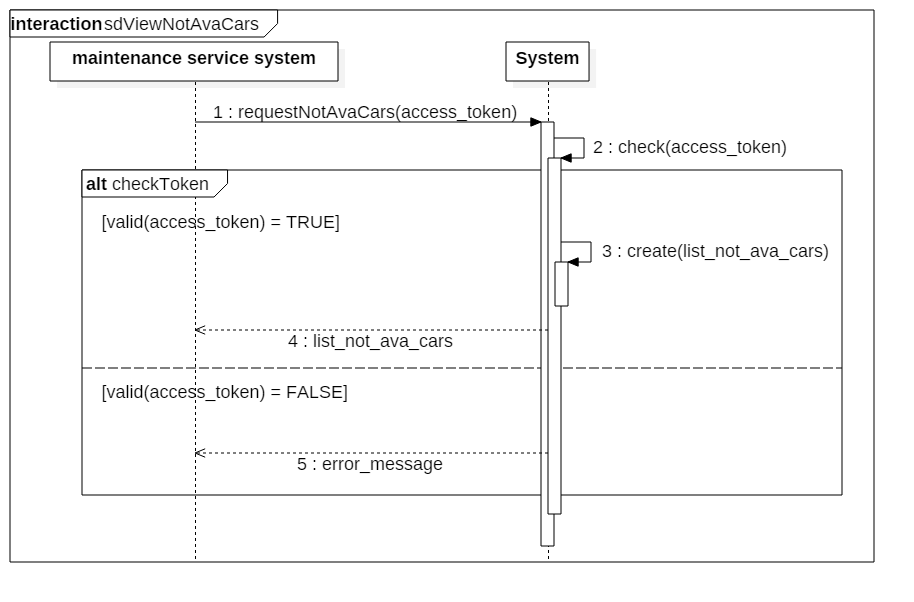
\includegraphics [width=\textwidth]{/diagrams/Sequence/sdViewNotAvaCars}
	\caption{
		\label{fig:visNotAvaSequence} 
		\emph{Visualization of not available cars} sequence diagram
	}
\end{figure}

%///////////////////////////////////////////////////////////
\clearpage
\subsubsection{Tag a car as available}
\begin{longtable}{p{0.25\linewidth}p{0.75\linewidth}}
\toprule
\textbf{Name} & \textbf{Tag a car as available} \\
\midrule
\textbf{Actors} &  Maintenance service system\\
\midrule
\textbf{Entry conditions} & Maintenance service system must know the access token to be identified by the system\\
\midrule
\textbf{Flow of events} & 
\begin{enumerate}
	\item The maintenance service system asks to tag a car as Available sending the car identifier
	paired with the access token
	\item The system checks the access token sent by the maintenance service
	\item The system checks the identifier received corresponds to a car with state set as \emph{Not Available}
	\item The system checks if the car identified by the identifier received is locked
	\item The system set the state of the car identified by the aforementioned identifier as \emph{Available}
	\item The system sends to the maintenance service system a confirmation message the car state has been set as \emph{Available}
\end{enumerate} \\
\midrule
\textbf{Exit conditions} & The car state is set as \emph{Available} \\
\midrule
\textbf{Exceptions} & 
\begin{itemize}
	\item If the access token sent by the maintenance service system is not recognized, the system sends to the maintenance service system an error message
	\item If the car identifier sent by the maintenance service system is not recognized or doesn't correspond to a car set as \emph{Not Available}, the system sends to the maintenance service system an error message
	\item If the car identifier sent by the maintenance service system corresponds to a car not locked, the system sends to the maintenance service system an error message
\end{itemize} \\
\bottomrule
\caption{\emph{Tag a car as not available} use case description}
\end{longtable}

\begin{figure}[h!]
	\centering
	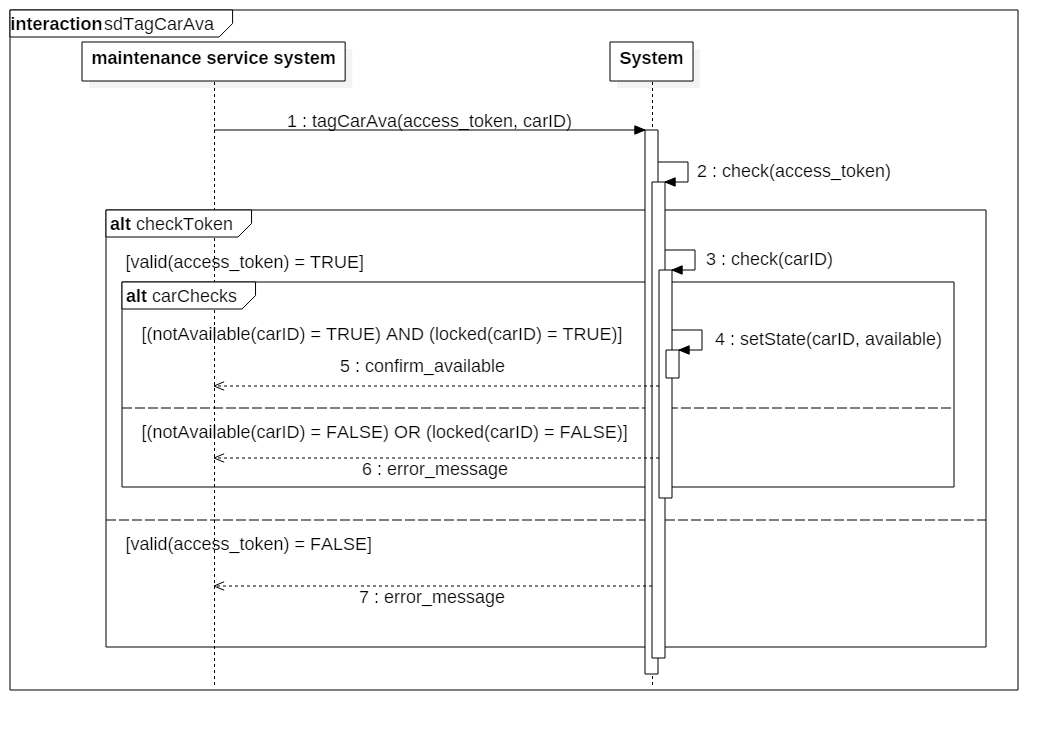
\includegraphics [width=\textwidth]{/diagrams/Sequence/sdTagCarAva}
	\caption{
		\label{fig:tagAvaSequence} 
		\emph{Tag a car as available} sequence diagram
	}
\end{figure}
%///////////////////////////////////////////////////////////
\clearpage
\subsubsection{Visualization of users information}
\begin{longtable}{p{0.25\linewidth}p{0.75\linewidth}}
\toprule
\textbf{Name} & \textbf{Visualization of users information} \\
\midrule
\textbf{Actors} &  Customer care operator\\
\midrule
\textbf{Entry conditions} & \\
\midrule
\textbf{Flow of events} & 
\begin{enumerate}
	\item The customer care operator inserts the username or the mail of a registered user
	\item The system checks if the username or the mail correspond to a user registered to the
	system
	\item The system retrieves user's data (name, surname, birth date and place, current domicile
	and driving license information) along with information about the car state the user is
	actually paired with
	\item The system shows to the customer care operator the info about the user
\end{enumerate} \\
\midrule
\textbf{Exit conditions} & The customer care operator can view the information required about the user \\
\midrule
\textbf{Exceptions} & 
\begin{itemize}
	\item If no users are found according to the parameters inserted by the customer care operator the system shows an error message
\end{itemize} \\
\bottomrule
\caption{\emph{Visualization of users information} use case description}
\end{longtable}

%///////////////////////////////////////////////////////////
\clearpage
\subsubsection{View users payments and rents history}
\begin{longtable}{p{0.25\linewidth}p{0.75\linewidth}}
\toprule
\textbf{Name} & \textbf{View users payments and rents history} \\
\midrule
\textbf{Actors} &  Customer care operator\\
\midrule
\textbf{Entry conditions} & \\
\midrule
\textbf{Flow of events} & 
\begin{enumerate}
	\item \textbf{Visualization of users information}
	\item The customer care operator asks to view user's payments and rents history
	\item The system retrieves the list of user's payments (successful and unsuccessful)
	\item The system retrieves the list of user's rents
	\item The system shows to the customer care operator user's payments and rents history
\end{enumerate} \\
\midrule
\textbf{Exit conditions} & The customer care operator can view the information required about the user \\
\midrule
\textbf{Exceptions} & \\
\bottomrule
\caption{\emph{View users payments and rents history} use case description}
\end{longtable}

%///////////////////////////////////////////////////////////
\clearpage
\subsubsection{Mark or unmark a user as banned}
\begin{longtable}{p{0.25\linewidth}p{0.75\linewidth}}
\toprule
\textbf{Name} & \textbf{Mark or unmark a user as banned} \\
\midrule
\textbf{Actors} &  Customer care operator\\
\midrule
\textbf{Entry conditions} & \\
\midrule
\textbf{Flow of events} & 
\begin{enumerate}
	\item The customer care operator inserts the username of a registered user
	\item The customer care operator asks to ban or to enable the registered user paired with the inserted username
		\begin{itemize}
			\item If the operator wants to mark a user as \emph{banned} he must insert a brief description of reasons why  
		\end{itemize}		 
	\item The system checks if the username corresponds to a user registered to the system
	\item The system marks or unmarks the user paired with the username as \emph{banned}
\end{enumerate} \\
\midrule
\textbf{Exit conditions} & The state of the user is updated \\
\midrule
\textbf{Exceptions} & 
\begin{itemize}
	\item If the username inserted by the customer car operator is not recognized, the system shows an error message
\end{itemize} \\
\bottomrule
\caption{\emph{Mark or unmark a user as banned} use case description}
\end{longtable}

%///////////////////////////////////////////////////////////
\clearpage
\subsubsection{Tag a car as not available}
\begin{longtable}{p{0.25\linewidth}p{0.75\linewidth}}
\toprule
\textbf{Name} & \textbf{Tag a car as not available} \\
\midrule
\textbf{Actors} &  Customer care operator\\
\midrule
\textbf{Entry conditions} & \\
\midrule
\textbf{Flow of events} & 
\begin{enumerate}
	\item The customer care operator inserts the identifier of the car
	\item The customer care operator asks to mark the car as \emph{Not Available}
	\item The customer care operator inserts a brief description of why the car state must be set as \emph{Not Available}
	\item The system checks the car identifier
	\item The system set the state of the car identified by the aforementioned identifier as \emph{Not Available} paired with the description
	\item The system shows a confirmation message the car has been tagged as \emph{Not Available}
\end{enumerate} \\
\midrule
\textbf{Exit conditions} & The state of the car is setted as \emph{Not Available}\\
\midrule
\textbf{Exceptions} & 
\begin{itemize}
	\item If car identifier sent by the customer care operator is not recognized, the system displays an error message
\end{itemize} \\
\bottomrule
\caption{\emph{Tag a car as not available} use case description}
\end{longtable}

\begin{figure}[h!]
	\centering
	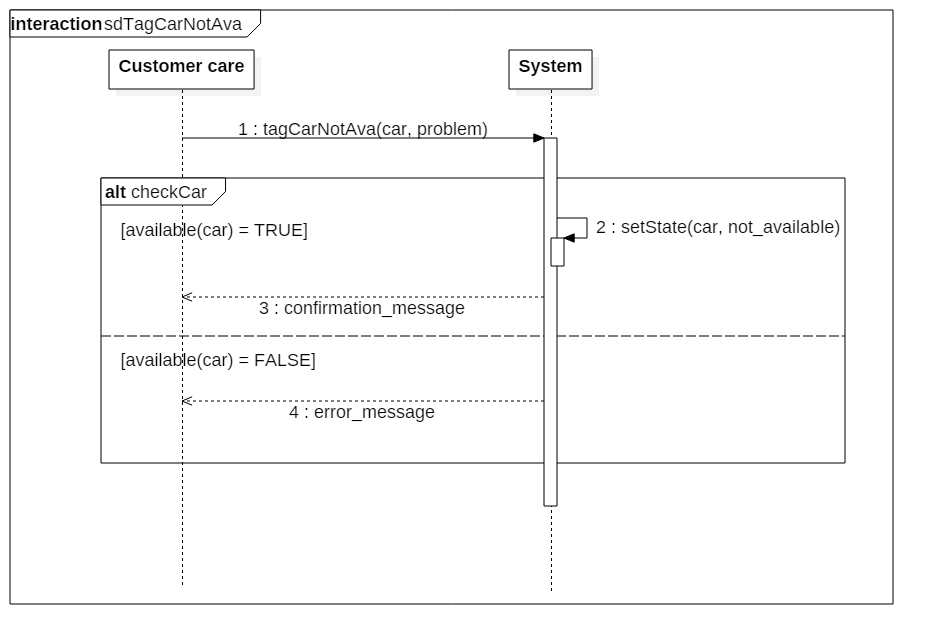
\includegraphics [width=\textwidth]{/diagrams/Sequence/sdTagCarNotAva}
	\caption{
		\label{fig:notAvaSequence} 
		\emph{Tag a car as Not Available} sequence diagram
	}
\end{figure}
\clearpage
\subsection{UML class diagram}
Based on collected scenarios and on the identified use cases we have developed the following requirements-level class diagram\cite{TextualAnalysis}. To ensure a better readability class attributes are not represented.
\begin{figure}[h!]
	\centering
	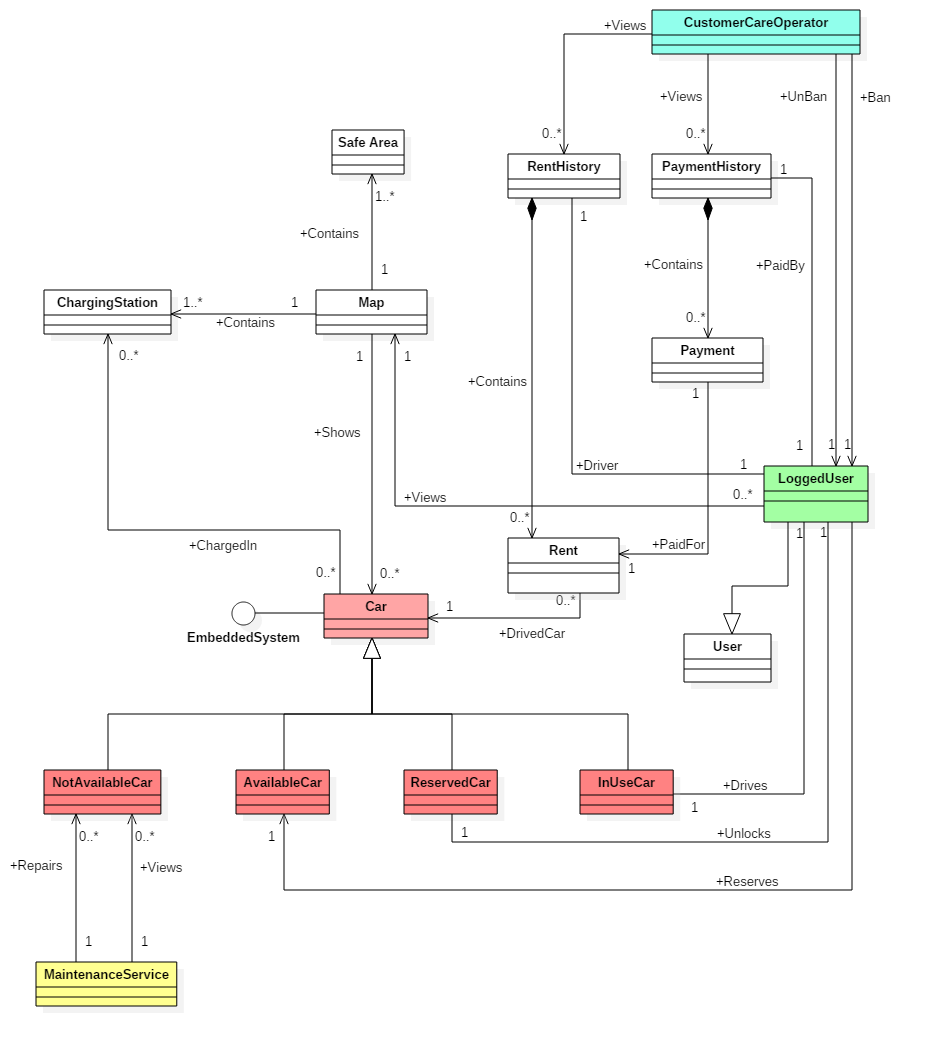
\includegraphics [width=\textwidth]{/diagrams/ClassDiagram}
	\caption{
		\label{fig:classDiagram} 
		UML class diagram
	}
\end{figure}

\begin{appendices}

	\section{Alloy model}
		\subsection{Source code}
		\lstinputlisting[language=alloy]{alloy/alloy2.0version.als}
		\begin{figure}[h!]
			\centering
			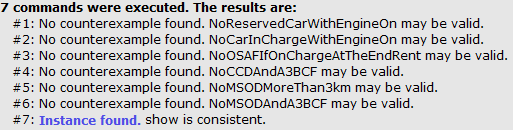
\includegraphics[]{alloy/AlloyResult.png}
			\caption{
				\label{fig:alloyExecutionResult} 
				Alloy execution result
			}
		\end{figure}
		\clearpage
		\subsection{Generated worlds}
			Note that in \autoref{fig:alloyWorld1} LoggedUser3 has been banned \emph{after} completing RentMade0.
			\begin{figure}[h!]
			\centering
			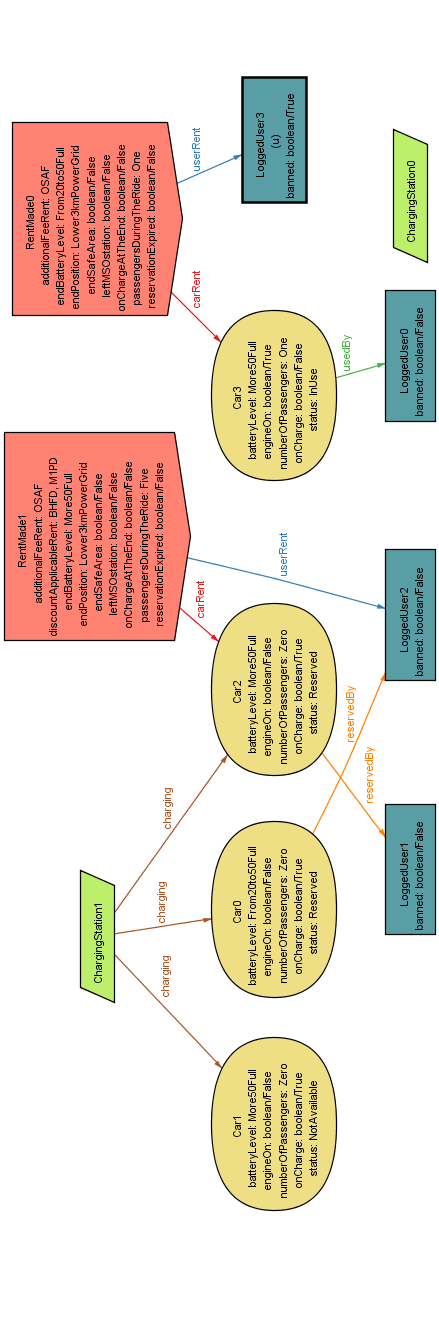
\includegraphics[scale=0.39]{alloy/AlloyWorld2.png}
			\caption{
				\label{fig:alloyWorld1} 
				First alloy generated world
			}
		\end{figure}
		\clearpage
		Note that in \autoref{fig:alloyWorld2} RentMade1 is actually a reservation expired of Car3 made by LoggedUser2. He now has reserved Car1.
		\begin{figure}[h!]
		\centering
		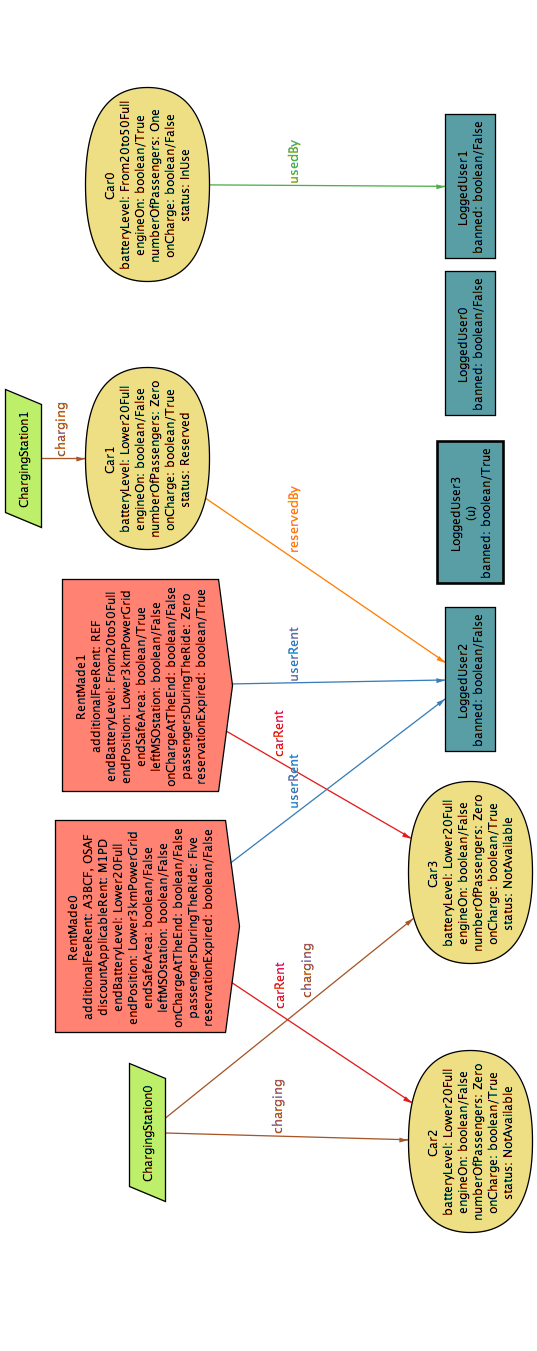
\includegraphics[scale=0.39]{alloy/AlloyWorld1.png}
		\caption{
			\label{fig:alloyWorld2} 
			Second alloy generated world
		}
		\end{figure}
		\clearpage
	\section{Software and tools used}
	For the development of this document we used
	\begin{itemize}
		\item \LaTeX{} as document preparation system
		\item \href{http://github.com}{GitHub} as version control system
		\item \href{http://draw.io}{Draw.io} for graphs
	\end{itemize}
		
	\section{Hours of Work}
	This is the amount of time spent to redact this document:
	\begin{itemize}
		\item \textbf{Section 1 - Introduction}
		\begin{itemize}
			\item Amedeo Cavallo - 2 hours
			\item Mattia Calabrese - 1 hour
			\item Federico Capaccio - 1 hour
		\end{itemize}
	\end{itemize}
	
	\section{Changelog}
	\begin{itemize}
		\item \textbf{v1.0} October 23, 2019
		\begin{itemize}
			\item Initial RASD document structuring and redaction
			\item Introduction (Purpose and Scope sections)
		\end{itemize}
	\end{itemize}
\end{appendices}
\clearpage
\begin{thebibliography}{9}
\bibitem{RE}B. Nuseibeh, S. Easterbrook, \emph{Requirements Engineering: A Roadmap}, 2000
\bibitem{Zave}P. Zave, \emph{Classification of Research Efforts in Requirements
Engineering}, ACM Computing Surveys, 1997
\bibitem{Assignments} E. Di Nitto, L. Mottola, \emph{Software Engineering 2 Assignment}, AA 2019-2020
\bibitem{Stone} A. Stone, “Chain of custody: How to ensure digital evidence stands up in court,” September 2015
\bibitem{IeeeRasd}IEEE Std 830:1993, \emph{IEEE Recommended Practice for Software Requirements Specifications}, 1993
\end{thebibliography}

\end{document}
